\chapter{Analisi Malware Chrysalis}

\subsection*{Studenti}
\begin{itemize}
  \item De Lucia Simone M63001720
  \item Covone Gabriel M63001809
\end{itemize}

\section{Descrizione}
Nel febbraio 2026 il gruppo di ricerca di Rapid7 fa luce su una campagna malware attribuita al gruppo APT Lotus Blossom che coinvolge il meccanismo di update automatici dell'applicazione di note Notepad++, rivelandosi di fatto un attacco supply chain. In particolare, la campagna ha avuto vari step tra cui:
\begin{itemize}
  \item la compromissione dei sistemi di rilascio degli update, accedendo in maniera non autorizzata ai sistemi di rilascio degli update.
  \item dirottare selettivamente alcuni traffici verso la risorsa mediante file manifest XML customizzati, costringendo così a forzare il software degli update automatici usato da Notepad++, in questo caso WinGUp.
  \item installare su target specifici dei pacchetti compromessi, sfruttando l'assenza di meccanismi di controllo dell'integrità crittografica nelle versioni del client WinGUp precedenti alla 8.8.9.
\end{itemize}

La campagna malware ha avuto una finestra temporale di circa 5 mesi, dal settembre 2025 al gennaio 2026; le vittime si concentravano in organizzazioni governative, istituzioni finanziarie e fornitori di servizi IT. In particolare, sono state colpite:
\begin{itemize}
  \item Un'organizzazione governativa nelle Filippine.
  \item Un fornitore di servizi IT in Vietnam.
  \item Un'istituzione finanziaria in El Salvador.
  \item Singoli utenti tecnici localizzati in Vietnam, Australia ed El Salvador.
\end{itemize}

Durante questo periodo, il malware ha operato in maniera silenziosa in tutti i sistemi infetti, effettuando information gathering e ottenendo accessi a sistemi critici in maniera remota. Inoltre, sono state trovate varie tipologie di loader e di servizi URL legati all'attacco in sé.

\begin{figure}[H]
  \centering
  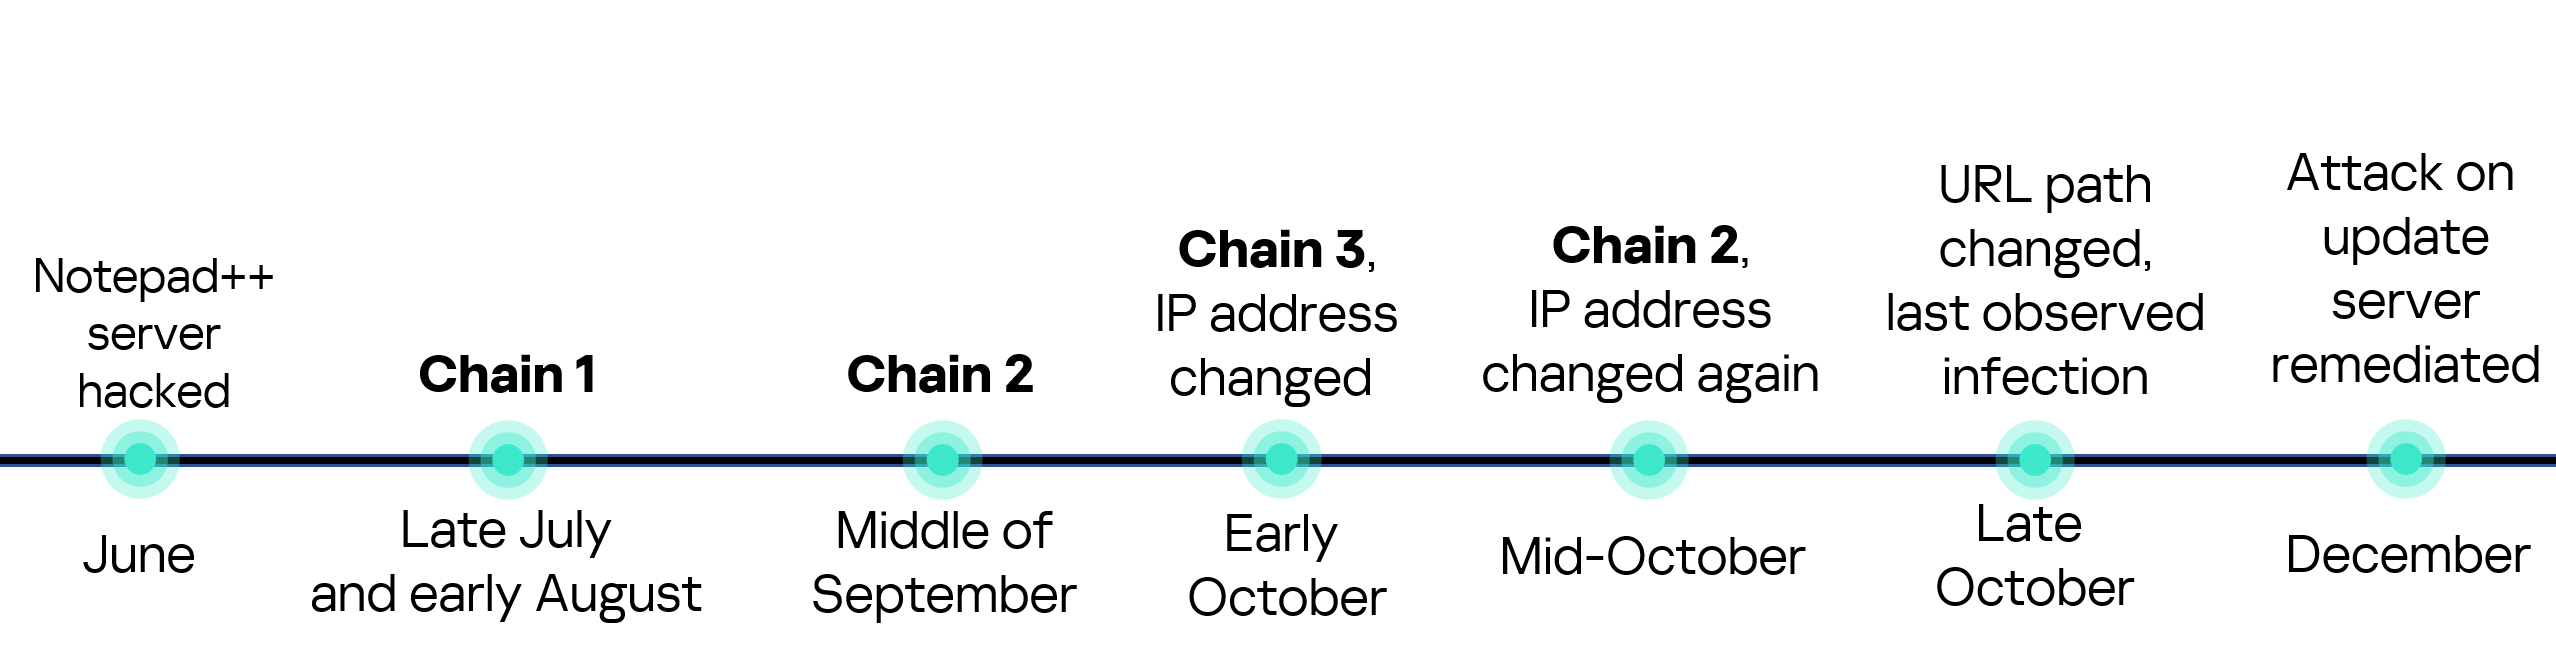
\includegraphics[width=0.85\textwidth]{img/notepad-supply-chain-attack-3-scaled.png}
  \caption{Monitoraggio campagna giugno/dicembre}
\end{figure}

\subsection{Chrysalis}
Durante questa campagna, l'ultimo malware utilizzato è stato rinominato Chrysalis.
La sua caratteristica principale risiede nel meccanismo di persistenza e di sofisticatezza del tool, oltre che a tanti strumenti di offuscamento. Dal punto di vista delle analisi, il malware è stato visto come uno step in avanti rispetto alle capacità pregresse del gruppo APT Lotus Blossom, e il chiaro intento di usare il malware per gestire una rete di informazioni da host infetti con uno strumento avanzato.

\section{Analisi}
Chrysalis è un malware backdoor che viene distribuito tramite un installer NSIS compromesso (\texttt{update.exe}), ottenuto grazie alla compromissione di WinGUp e alla catena di approvvigionamento degli update automatici.

\subsection{Tool Utilizzati}
I tool utilizzati sono suddivisi in base alla fase operativa per intercettare, decodificare e sconfiggere i meccanismi di evasione del malware:

\begin{table}[H]
\centering
\begin{tabular}{|l|l|p{8cm}|}
\hline
\textbf{Fase} & \textbf{Strumenti} & \textbf{Scopo Principale} \\ \hline
\textbf{1. Triage e Analisi Statica} & PEstudio, PEview, capa & Ispezione degli header PE, controllo dell'entropia/offuscamento e analisi iniziale delle capability delle API. \\ \hline
\textbf{2. Monitoraggio e Simulazione} & Procmon, FakeNet-NG, Wireshark & Monitoraggio in tempo reale del comportamento locale (registro/file) e simulazione del traffico di rete verso il C2. \\ \hline
\textbf{3. Debugging e Memory Dumping} & x32dbg, ScyllaHide, Scylla, PE-bear & Esecuzione controllata passo-passo, evasione delle difese anti-debug, dumping del payload e ricostruzione della IAT. \\ \hline
\textbf{4. Reverse Engineering e IoC} & IDA Freeware 8.2, FLOSS, yarGen & Decompilazione per lo studio della logica interna del malware, de-offuscamento automatico delle stringhe e creazione di regole YARA. \\ \hline
\end{tabular}
\caption{Fasi operative e strumenti utilizzati durante l'analisi.}
\end{table}

\section{Esecuzione del malware e Indicatori di Compromissione (IoC)}
Il primo step è stato fatto per raccogliere informazioni relative al malware, sia dal punto di vista di report online e di analisi, sia come opera all'interno di un sistema infetto. Questo non solo ci permette di consolidare le informazioni lette, ma anche di approfondire vari aspetti dell'infezione.

Si è partiti con l'esecuzione dell'update malevolo, per poi analizzare il comportamento scaturito all'interno dell'host.

\subsection{File creati nell'host}
Una volta avviato l'update malevolo, all'interno del disco di sistema viene creata la cartella \texttt{\%appdata\%\textbackslash Roaming\textbackslash Bluetooth\textbackslash} contenente i vari file malevoli che andranno a costituire la catena di esecuzione del malware.

\begin{figure}[H]
  \centering
  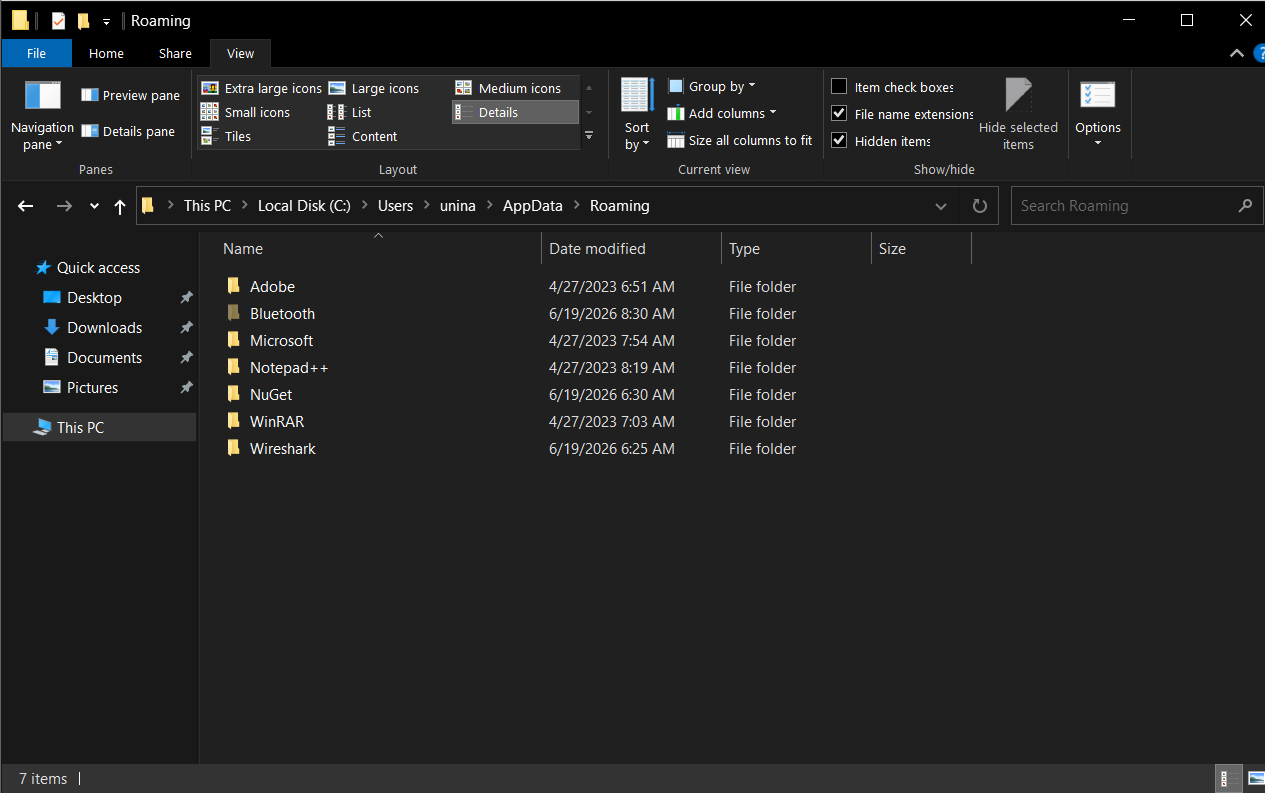
\includegraphics[width=0.7\textwidth]{img/appdata_roaming.png}
  \caption{Cartella AppData Roaming}
\end{figure}

\begin{figure}[H]
  \centering
  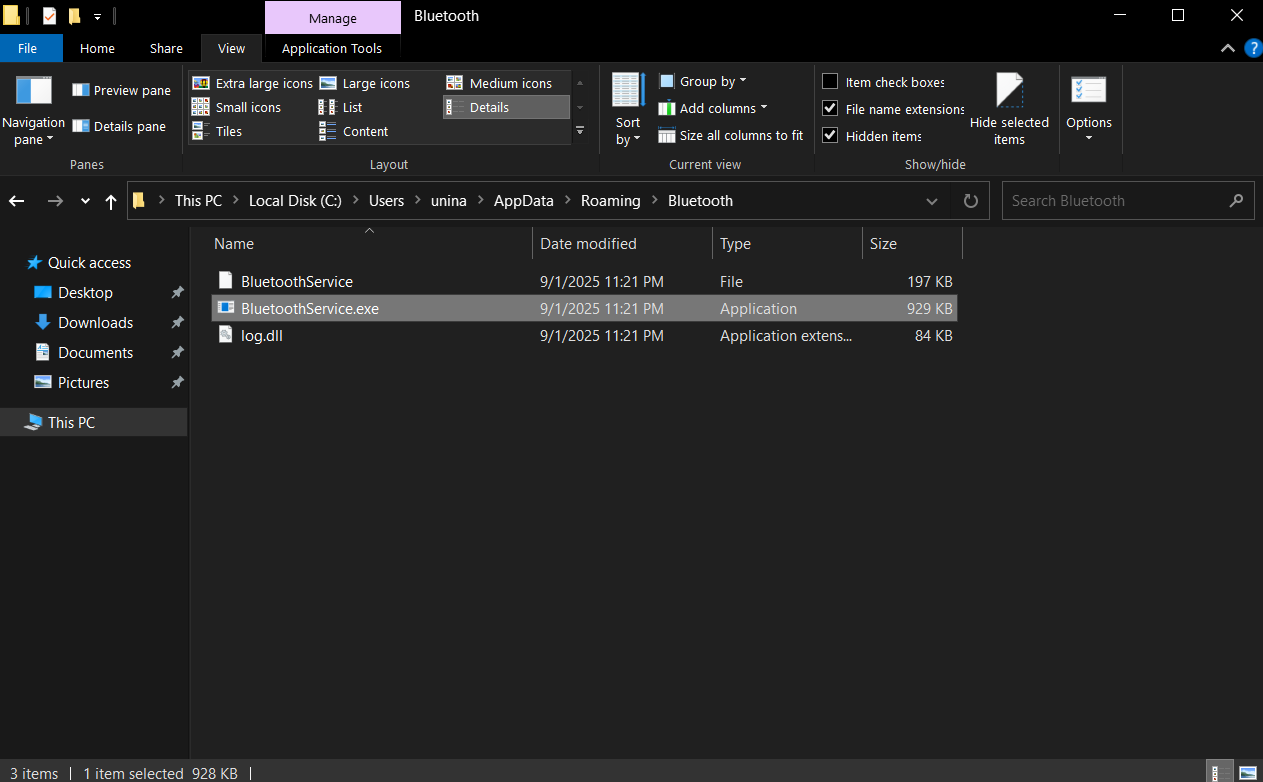
\includegraphics[width=0.7\textwidth]{img/bluetoothFolder.png}
  \caption{Contenuto Cartella Bluetooth}
\end{figure}

Vengono identificati tre file, di cui ne analizziamo l'entropia e le proprietà:
\begin{itemize}
  \item \textbf{\texttt{BluetoothService.exe}}: L'eseguibile in sé è legittimo, tuttavia possiamo notare che la firma è stata modificata. In realtà risulta essere un servizio BitDefender. Eventuali ricerche hanno portato alla luce che normalmente può effettuare side-loading di una libreria di logging.
  \begin{figure}[H]
    \centering
    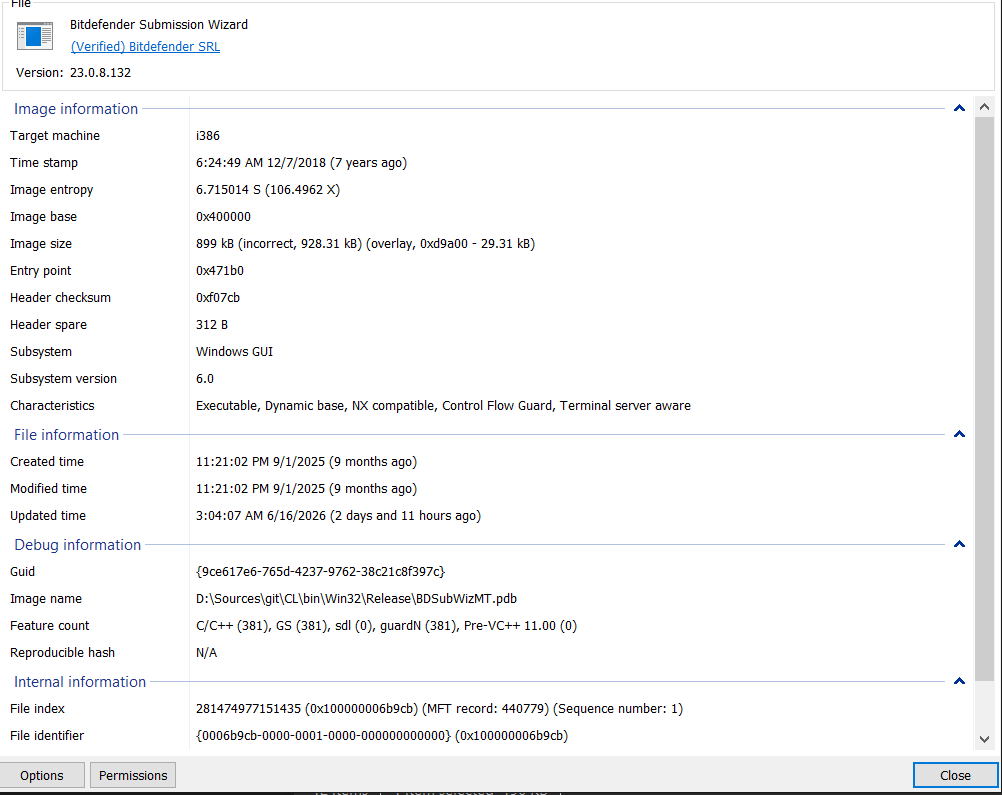
\includegraphics[width=0.7\textwidth]{img/FirmaModificataBluetoothService.png}
    \caption{Proprietà di \texttt{BluetoothService.exe}}
  \end{figure}
  \item \textbf{\texttt{log.dll}}: La libreria appare legittima, tuttavia viene notata un'entropia abbastanza elevata nella sezione di testo, simbolo che ci sia del codice cifrato.
  \begin{figure}[H]
    \centering
    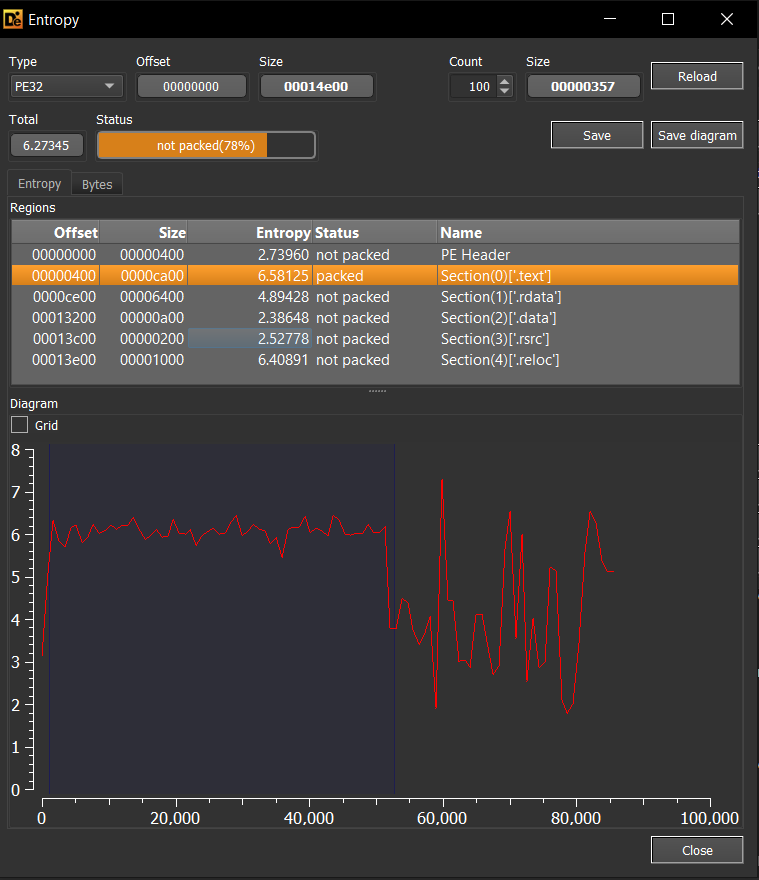
\includegraphics[width=0.7\textwidth]{img/Entropylog.png}
    \caption{Entropia DLL}
  \end{figure}
  \item \textbf{\texttt{BluetoothService}}: Il file è cifrato ed è senza estensione, è lo shellcode vero e proprio.
  \begin{figure}[H]
    \centering
    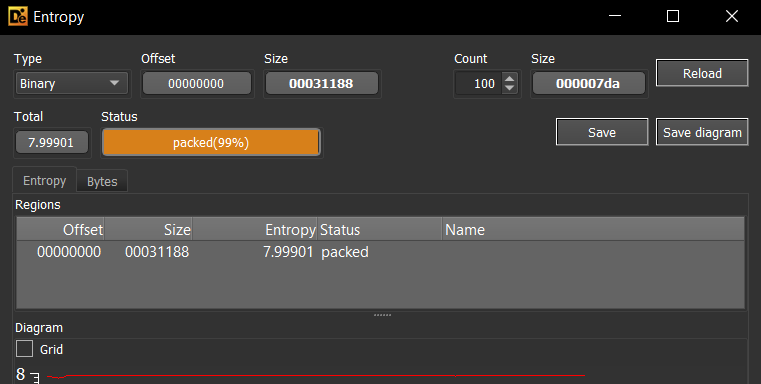
\includegraphics[width=0.7\textwidth]{img/BluetoothServiceEntropy.png}
    \caption{Entropia ShellCode}
  \end{figure}
\end{itemize}

\subsection{Connessioni all'esterno e Traffico C2}
Un altro passaggio è stato il setup di FakeNet-NG e di Wireshark per intercettare eventuali richieste che provengono dall'esterno.
Una volta avviato, è possibile notare che il malware tenta di stabilire una connessione HTTPS cifrata verso il proprio server C2.

\begin{figure}[H]
  \centering
  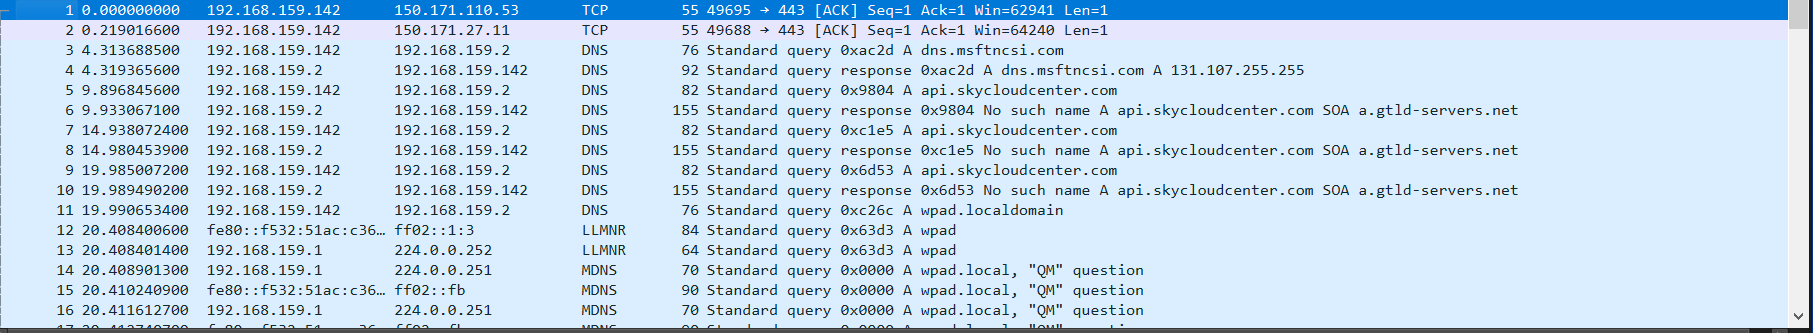
\includegraphics[width=0.85\textwidth]{img/Wireshark_Traffic_Capture.png}
  \caption{Wireshark Traffic Capture}
\end{figure}

Grazie a FakeNet-NG, è stato possibile intercettare alcune richieste POST HTTP, con i seguenti dettagli principali:
\begin{itemize}
  \item \textbf{Host remoto}: \texttt{api.skycloudcenter.com}
  \item \textbf{Indirizzo IP reale di C2 (Threat Intelligence)}: L'analisi del traffico reale e i report di intelligence collegano il dominio \texttt{api.skycloudcenter.com} del gruppo Lotus Blossom principalmente a:
  \begin{itemize}
    \item È stato rinvenuto un indirizzo IP \textbf{\texttt{61.4.102.97}}, geolocalizzato in Malesia, ma ritenuto benevolo.
  \end{itemize}
  Non è stato possibile ottenere ulteriori indirizzi, siccome le query DNS non hanno dato riscontro.
  \item \textbf{Struttura della richiesta POST} estratta tramite FakeNet-NG:
\begin{lstlisting}[language=HTML]
POST /a/chat/s/70521ddf-a2ef-4adf-9cf0-6d8e24aaa821 HTTP/1.1
Host: api.skycloudcenter.com
User-Agent: Mozilla/5.0 (Windows NT 10.0; Win64; x64) AppleWebKit/537.36 (KHTML, like Gecko) Chrome/80.0.4044.92 Safari/537.36
Content-Type: text/html
\end{lstlisting}
  \item \textbf{Payload}: Il payload HTTP cifrato, indizio dell'uso di HTTPS per l'esfiltrazione dei dati.
\end{itemize}

\subsubsection{Monitoraggio processo per esfiltrazione dei dati}
Tramite Process Monitor è possibile confermare che l'origine del traffico proviene dal processo \texttt{BluetoothService.exe}.

\begin{enumerate}
  \item \textbf{Analisi del flusso TCP:}
  Questo conferma che \texttt{BluetoothService.exe} invia richieste verso l'IP di laboratorio \texttt{192.0.2.123} sulla porta \texttt{443} (HTTPS), che viene intercettata da FakeNet per l'esfiltrazione di dati. Il relativo payload rinvenuto da FakeNet risulta cifrato a causa dell'uso del protocollo di trasporto TLS/HTTPS.
  \begin{figure}[H]
    \centering
    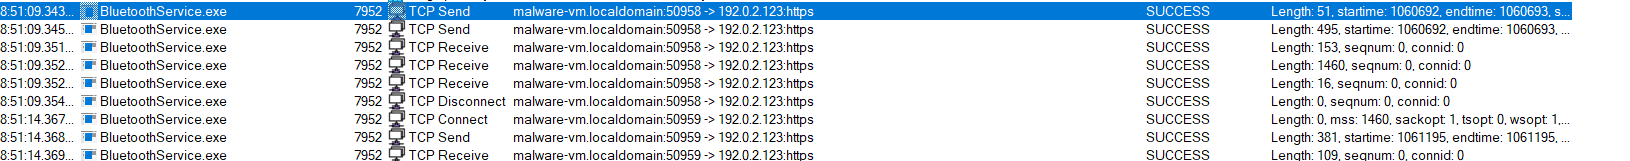
\includegraphics[width=0.85\textwidth]{img/tcp_traffic.png}
    \caption{Dettaglio del traffico TCP in Procmon}
  \end{figure}

  \item \textbf{Analisi dello Stack Trace e Deviazione del Traffico (\texttt{tcp\_send\_traffic.png}):}
  \begin{itemize}
    \item \textbf{Deviazione del traffico via WinDivert}: Lo stack trace dell'evento \texttt{TCP Send} rivela che il malware intercetta e inietta pacchetti a basso livello nel Windows Filtering Platform (\texttt{fwpkclnt.sys} tramite \texttt{FwpsStreamInjectAsync0}/\texttt{FwpsInjectNetworkSendAsync0} e \texttt{Wdf01000.sys}), bypassando le API socket standard (\texttt{ws2\_32.dll}) tramite il driver \texttt{WinDivert64.sys}.
    \item \textbf{Indicatori di Packaging (PyInstaller) ed Esecuzione}: La presenza del percorso temporaneo \texttt{\_MEIxxxxx} (es. \texttt{\_MEI28002}) indica che il malware è pacchettizzato in Python tramite PyInstaller, il quale scompatta a runtime il modulo \texttt{pydivert} e il rispettivo driver. Lo user-mode stack evidenzia inoltre un'esecuzione a 32 bit in ambiente WoW64, con caricamento del driver direttamente durante l'inizializzazione del thread.
  \end{itemize}
  \begin{figure}[H]
    \centering
    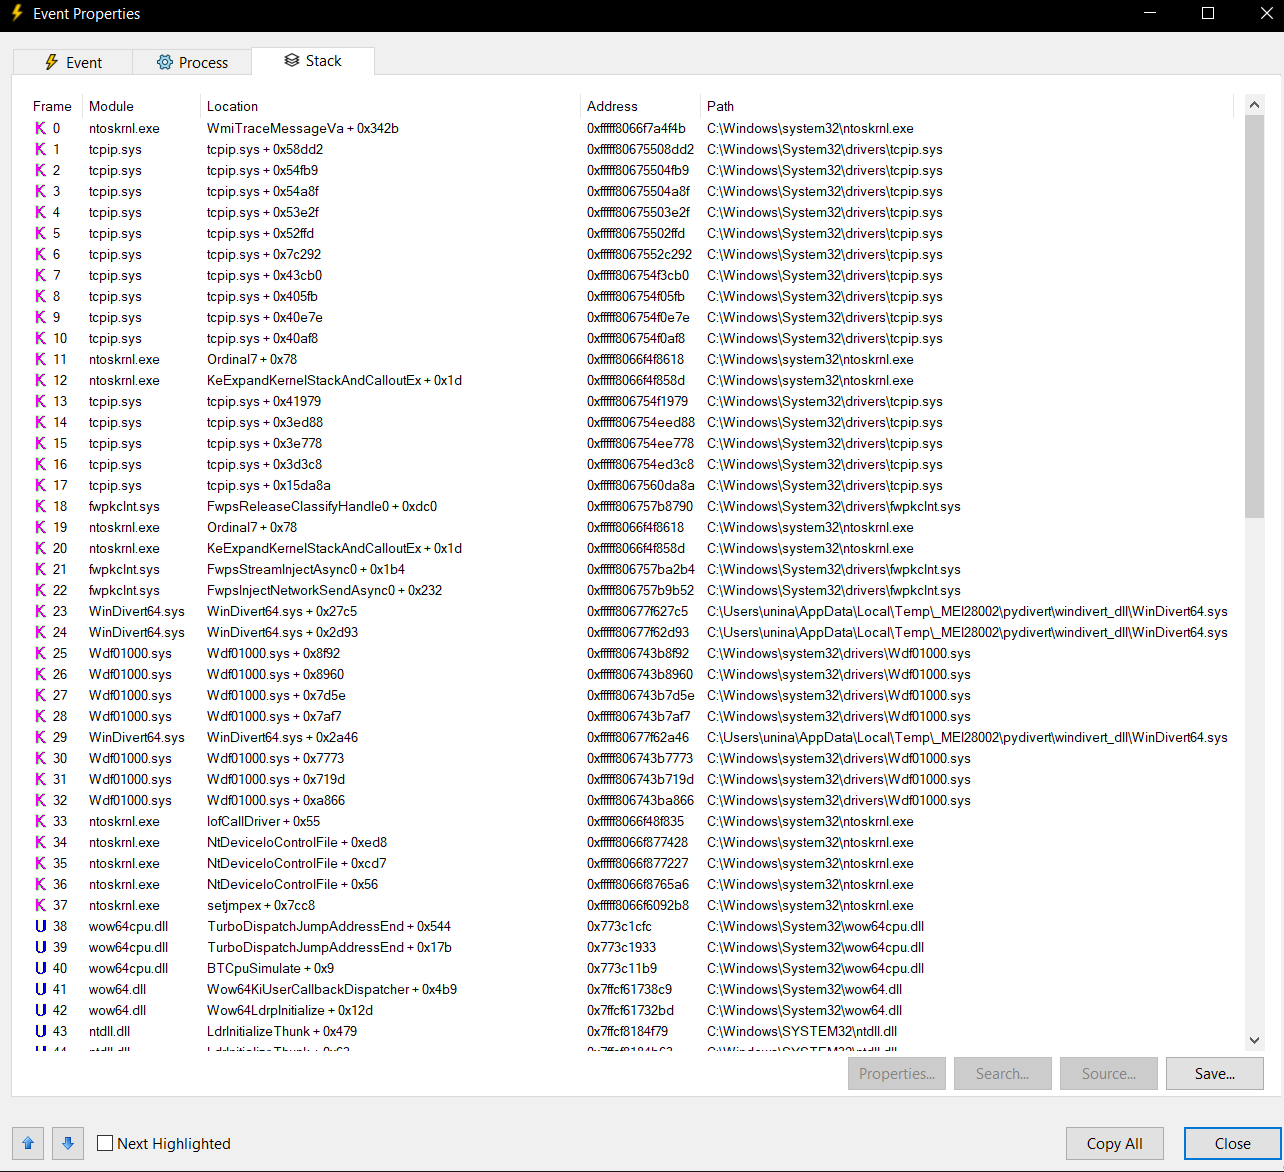
\includegraphics[width=0.85\textwidth]{img/tcp_send_traffic.png}
    \caption{Stack Trace del TCP Send con WinDivert}
  \end{figure}
\end{enumerate}

\subsubsection{Persistenza e Chiavi di Registro}
Si può anche osservare che il malware registra un servizio di sistema denominato \texttt{BluetoothService} per garantirne l'esecuzione automatica ad ogni avvio dell'host. Questo servizio viene riportato all'interno del registro di sistema.

\begin{figure}[H]
  \centering
  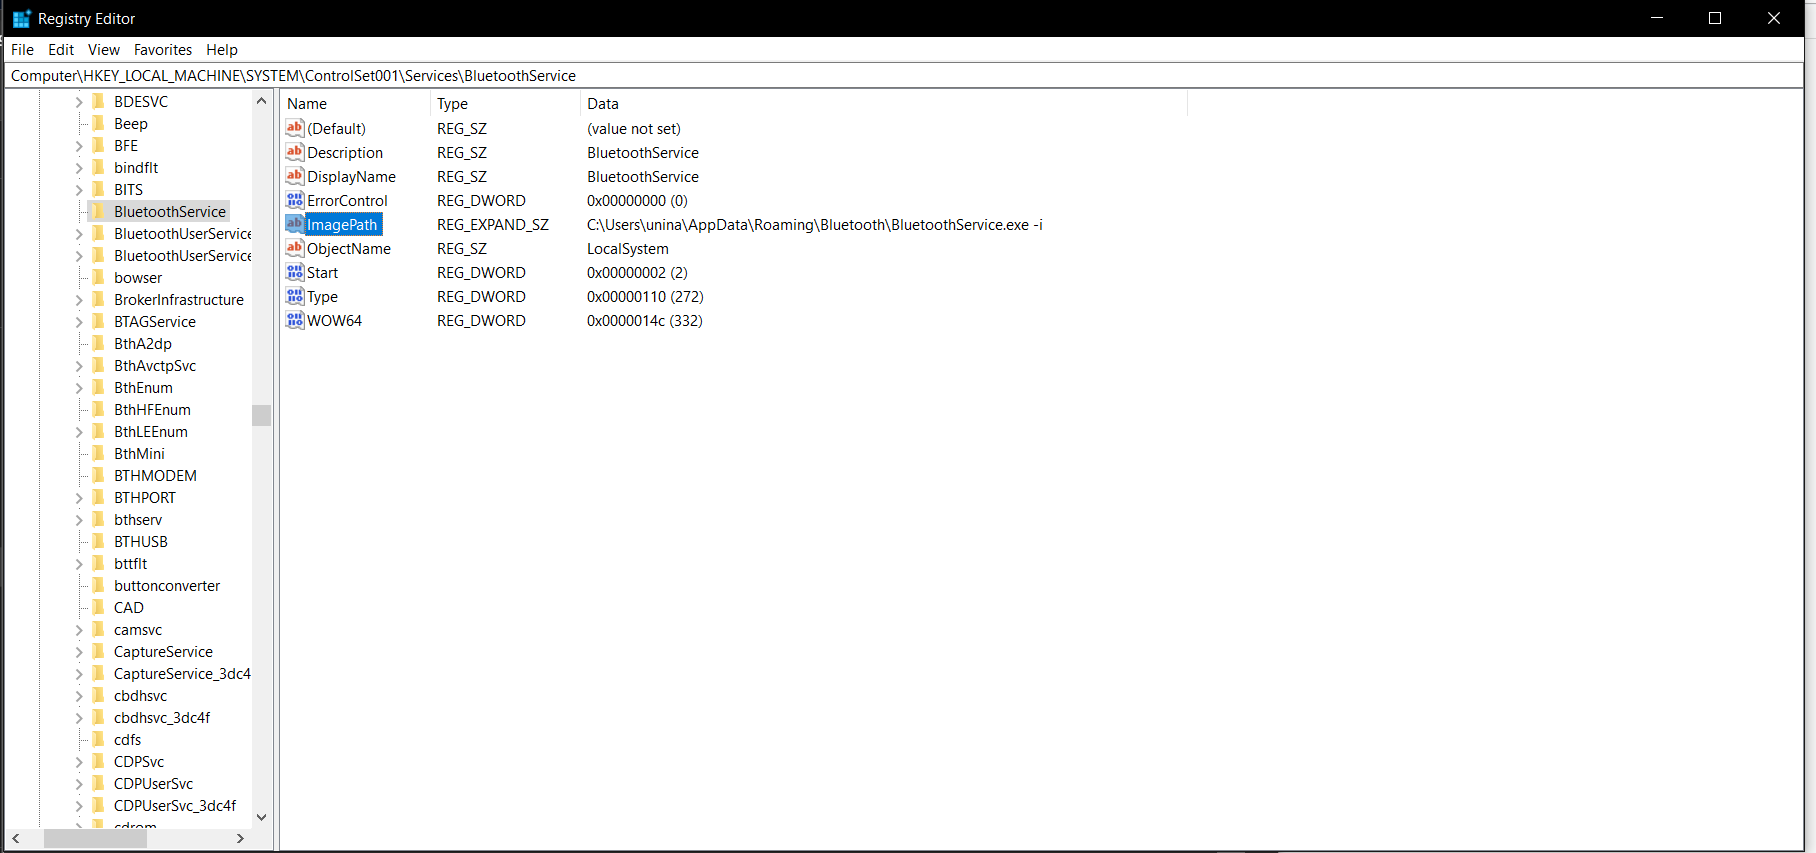
\includegraphics[width=0.85\textwidth]{img/bluetoothService_registry.png}
  \caption{Chiave di Registro \texttt{BluetoothService}}
\end{figure}

\begin{itemize}
  \item \textbf{Servizio creato}: \texttt{BluetoothService}
  \item \textbf{Chiave di registro}: \texttt{HKLM\textbackslash SYSTEM\textbackslash CurrentControlSet\textbackslash Services\textbackslash BluetoothService}
  \item \textbf{Comando di esecuzione}: \texttt{C:\textbackslash Users\textbackslash unina\textbackslash AppData\textbackslash Roaming\textbackslash Bluetooth\textbackslash BluetoothService.exe -i} (eseguito con privilegi di \texttt{LocalSystem}).
\end{itemize}

\begin{figure}[H]
  \centering
  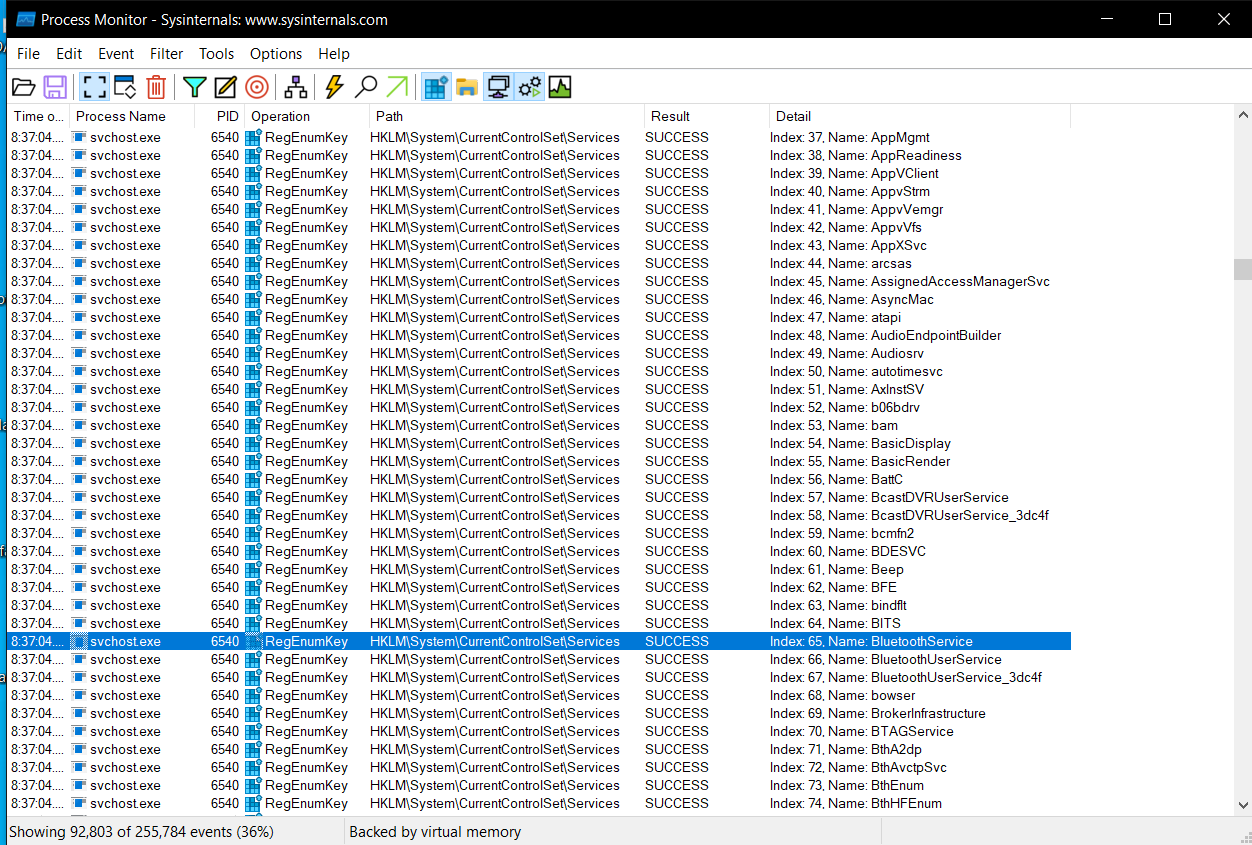
\includegraphics[width=0.85\textwidth]{img/Procmon_Registry_Service_Enum.png}
  \caption{Procmon Service Registry Enumeration}
\end{figure}

Inoltre, grazie a ProcMon, possiamo osservare che il processo di sistema \texttt{svchost.exe} (PID 6540) esegue un'operazione di enumerazione del registro (\texttt{RegEnumKey}) sotto \texttt{HKLM\textbackslash System\textbackslash CurrentControlSet\textbackslash Services}, caricando e individuando con successo la chiave del servizio \texttt{BluetoothService} creata dal malware (all'indice 65) per avviarne poi l'esecuzione di \texttt{BluetoothService.exe}.

Durante l'esecuzione, il malware effettua la profilazione del sistema leggendo l'identificativo univoco della macchina tramite la chiave:
\begin{itemize}
  \item \texttt{HKLM\textbackslash Software\textbackslash Microsoft\textbackslash Cryptography\textbackslash MachineGuid}
\end{itemize}

\begin{figure}[H]
  \centering
  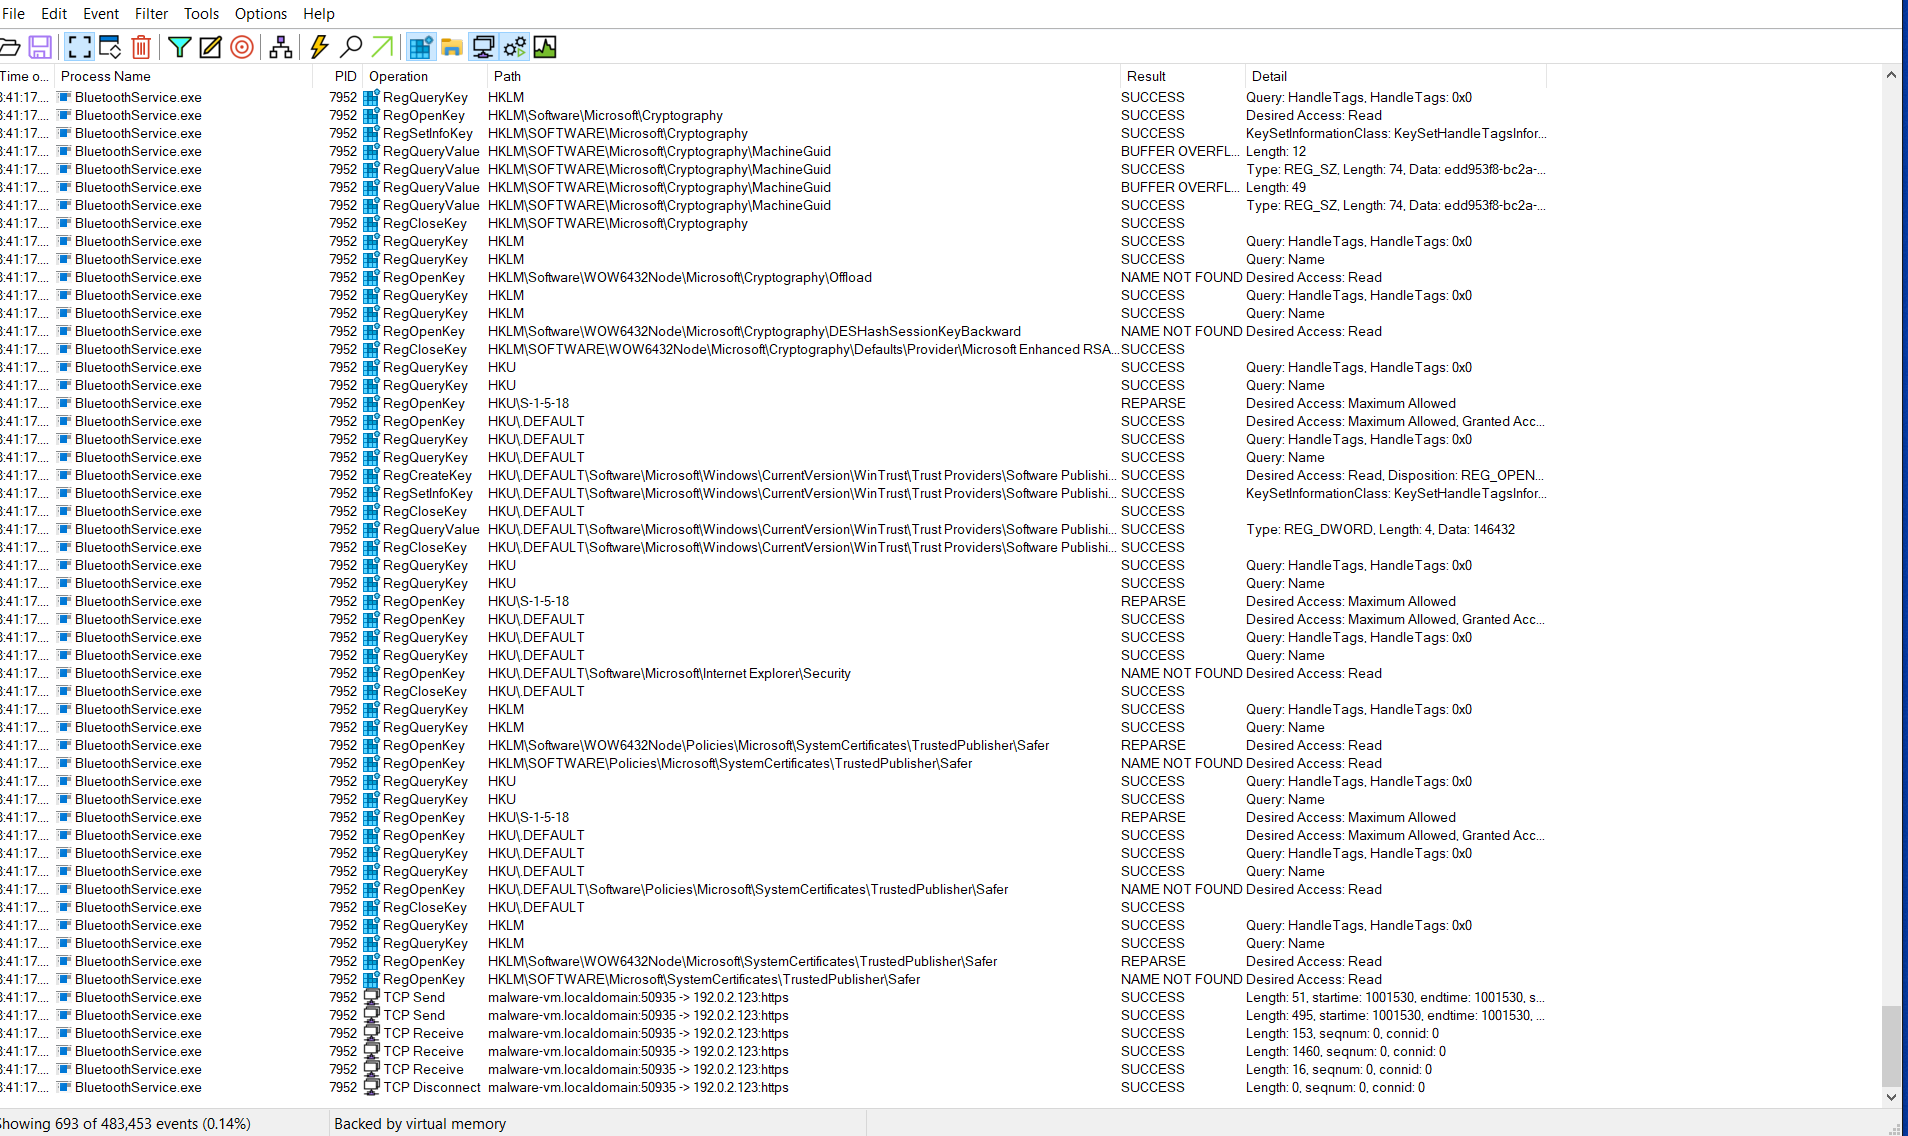
\includegraphics[width=0.85\textwidth]{img/Procmon_C2_HTTPS_Connection.png}
  \caption{Procmon MachineGuid e Traffico di Rete}
\end{figure}

\subsubsection{Evasione, Monitoraggio e Chiusura}
Durante il monitoraggio dell'esecuzione del malware tramite Process Monitor, si osserva la terminazione improvvisa del thread principale e del processo una volta completata l'iniezione, allo scopo di eludere l'analisi dinamica.

\begin{figure}[H]
  \centering
  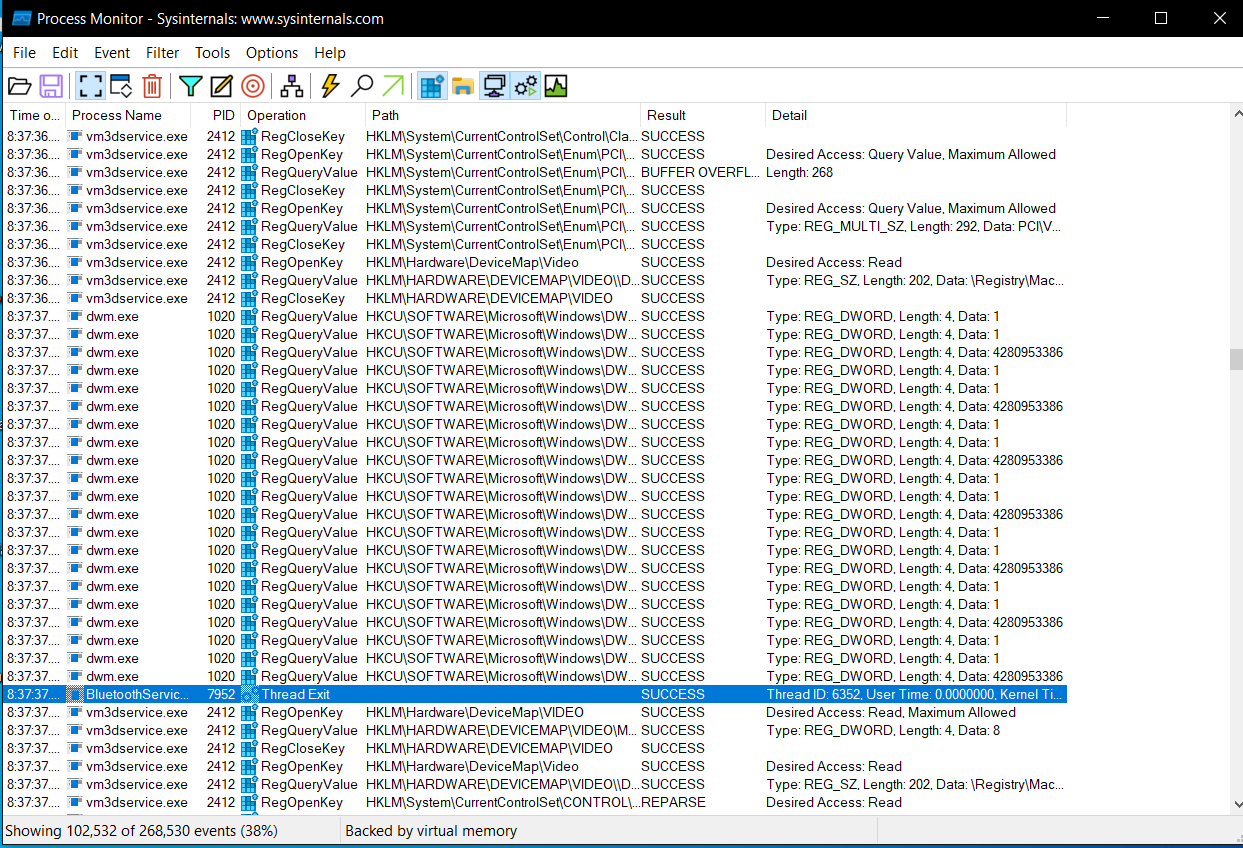
\includegraphics[width=0.85\textwidth]{img/Procmon_Thread_Exit.png}
  \caption{Procmon Thread Exit}
\end{figure}

\begin{figure}[H]
  \centering
  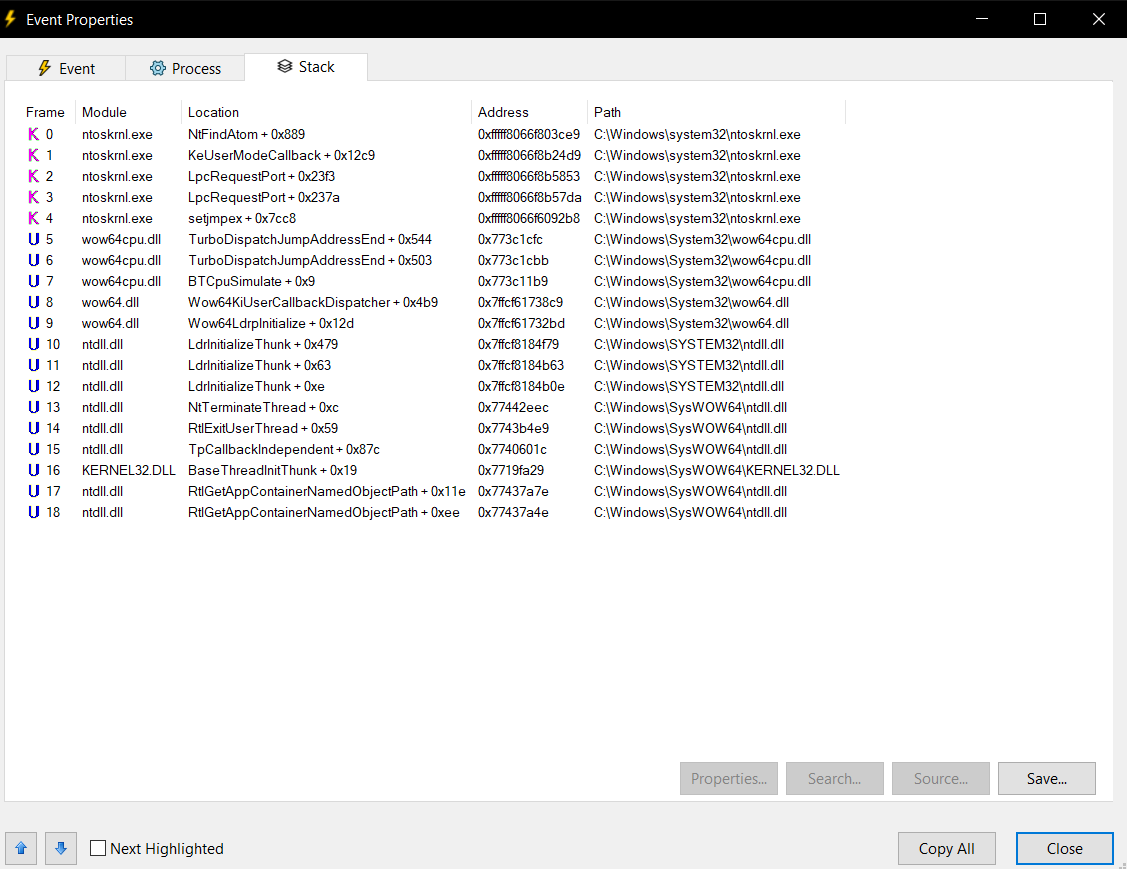
\includegraphics[width=0.85\textwidth]{img/Procmon_Stack_Trace_Thread_Exit.png}
  \caption{Stack Trace Thread Exit}
\end{figure}

La stack trace dell'evento di \texttt{Thread Exit} mostra come l'esecuzione passi attraverso le librerie \texttt{wow64cpu.dll} (\texttt{BTCpuSimulate}) e \texttt{ntdll.dll} (\texttt{NtTerminateThread}), a conferma del fatto che il malware avvia il proprio codice e poi termina il thread primario per disorientare i debugger.

\section{Roadmap di Analisi Operativa}
Possiamo confermare, quindi, che il malware è formato dalle seguenti componenti:

\begin{enumerate}
  \item \textbf{L'Installer NSIS (\texttt{update.exe})}: \texttt{sha256:8ea8b83645fba6e23d48075a0d3fc73ad2ba515b4536710cda4f1f232718f53e} \\
  Avvia l'infezione estraendo tre componenti principali all'interno della cartella \texttt{\%appdata\%\textbackslash Roaming\textbackslash Bluetooth\textbackslash}:
  \begin{itemize}
    \item \textbf{\texttt{BluetoothService.exe}} \texttt{sha256:2da00de67720f5f13b17e9d985fe70f10f153da60c9ab1086fe58f069a156924} (un eseguibile legittimo firmato da Bitdefender, originariamente \texttt{BDSubWizMT.exe}).
    \item \textbf{\texttt{log.dll}} \texttt{sha256:3bdc4c0637591533f1d4198a72a33426c01f69bd2e15ceee547866f65e26b7ad} (la libreria dinamica malevola).
    \item \textbf{\texttt{BluetoothService}} \texttt{sha256:77bfea78def679aa1117f569a35e8fd1542df21f7e00e27f192c907e61d63a2e} (il payload contenente lo shellcode offuscato, privo di estensione).
  \end{itemize}
  \item \textbf{DLL Sideloading}: All'avvio di \texttt{BluetoothService.exe}, il sistema operativo Windows carica automaticamente \texttt{log.dll} presente nella stessa cartella (sideloading).
  \item \textbf{Esecuzione dello Shellcode}: La funzione di inizializzazione di \texttt{log.dll} (\texttt{DllMain} / \texttt{LogInit}) legge il file \texttt{BluetoothService} crittografato dal disco, lo decritta in memoria RAM usando un algoritmo matematico custom e vi trasferisce l'esecuzione.
  \begin{itemize}
    \item \textbf{Comunicazione C2}: Il payload finale decrittato (backdoor Chrysalis) effettua la profilazione dell'host e si connette al server di Command and Control (C2) per l'esfiltrazione e la ricezione di comandi.
  \end{itemize}
\end{enumerate}

L'architettura del flusso di esecuzione è riassunta nel seguente diagramma:

\begin{figure}[H]
  \centering
  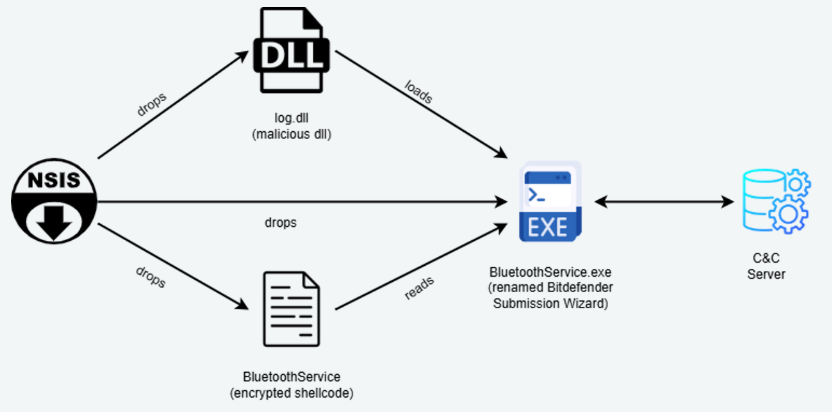
\includegraphics[width=0.85\textwidth]{img/chrysalis-execution.png}
  \caption{Architettura di esecuzione Chrysalis}
\end{figure}

\subsection{Analisi di Dettaglio dei Componenti e Ingegneria Inversa}

\subsubsection{update.exe (Dropper NSIS)}
\begin{itemize}
  \item \textbf{Tecnologia}: Archivio autoinstallante NSIS (Nullsoft Scriptable Install System).
  \item \textbf{Funzione principale}: Estrae i componenti malevoli nella directory di sistema \texttt{\%APPDATA\%\textbackslash Roaming\textbackslash Bluetooth\textbackslash}.
  \item \textbf{Tecniche di Evasione e Permessi NTFS Custom}:
  \begin{itemize}
    \item \textbf{DACL personalizzata}: La subroutine \texttt{sub\_405B06} definisce un descrittore di sicurezza personalizzato applicato alla cartella creata. Nello specifico, imposta una DACL con due ACE (Access Control Entries):
    \begin{enumerate}
      \item \textit{ACE 1}: Permessi di \texttt{ACCESS\_ALLOWED} su \texttt{BUILTIN\textbackslash Administrators} con flag \texttt{GENERIC\_ALL} (controllo completo).
      \item \textit{ACE 2}: Permessi di \texttt{ACCESS\_ALLOWED} su \texttt{Everyone} limitati esclusivamente a \texttt{READ\_CONTROL}, \texttt{FILE\_READ\_DATA}, \texttt{FILE\_DELETE\_CHILD} e \texttt{SYNCHRONIZE}. Questa configurazione impedisce modifiche o scritture successive ma consente la lettura e la cancellazione manuale del contenuto.
    \end{enumerate}
    \item \textbf{Attributi Hidden/System}: L'installer richiama l'API \texttt{SetFileAttributesW} per camuffare i file estratti sul file system. La funzione \texttt{sub\_401434} ricicla il parametro \texttt{nCmdShow} della funzione \texttt{WinMain} dell'eseguibile (tipicamente impostato a \texttt{2} o \texttt{6}) passandolo direttamente come \texttt{dwFileAttributes}. Se il valore corrisponde a tali costanti, i file e la cartella vengono configurati come nascosti o di sistema (\texttt{FILE\_ATTRIBUTE\_HIDDEN} o \texttt{HIDDEN|SYSTEM}), celandoli a ricerche visive superficiali da parte dell'utente.
    \item \textbf{Persistenza nel Registro}: L'archivio NSIS contiene uno script compilato (opcode \texttt{0x33}) che richiama \texttt{RegSetValueExW} per registrare il valore \texttt{BluetoothService} sotto la chiave di avvio automatico \texttt{HKCU\textbackslash Software\textbackslash Microsoft\textbackslash Windows\textbackslash CurrentVersion\textbackslash Run}, puntando all'eseguibile esca.
  \end{itemize}
\end{itemize}

\subsubsection{BluetoothService.exe (Loader \& Esca Sideloading)}
\begin{itemize}
  \item \textbf{Firma e Autenticità}: Originariamente l'eseguibile \texttt{BDSubWizMT.exe} (Bitdefender Submission Wizard), firmato digitalmente ma vulnerabile. Il malware lo utilizza come esca legittima per forzare il caricamento dinamico della libreria malevola presente nella stessa directory.
  \item \textbf{Flusso di Caricamento (\texttt{LogLoader\_Init})}:
  \begin{itemize}
    \item La subroutine \texttt{sub\_404760} recupera la directory in cui risiede l'eseguibile tramite \texttt{GetModuleFileNameW}.
    \item Sostituisce il nome dell'eseguibile nel percorso per concatenare ed individuare il file \texttt{log.dll}.
    \item Effettua il caricamento manuale della libreria tramite \texttt{LoadLibraryW(L"log.dll")}.
    \item Risolve dinamicamente le esportazioni di log richiamando \texttt{GetProcAddress} per le funzioni \texttt{LogInit}, \texttt{LogWrite}, \texttt{LogApplySettings}, e altre.
    \item Salva i puntatori a queste funzioni all'interno di una struttura globale (\texttt{dword\_4BCFBC}).
    \item Avvia l'esecuzione del malware richiamando immediatamente l'esportazione \texttt{LogInit()} risolta dal DLL.
  \end{itemize}
\end{itemize}

\subsubsection{log.dll (Loader Intermedio e API Hashing)}
\begin{itemize}
  \item \textbf{Falsi Metadati}: La DLL esporta funzioni con nomi fittizi tipici di librerie di logging per mascherare la sua natura malevola. Le funzioni risolte a runtime sono:
  \begin{itemize}
    \item \texttt{LogInit}: Inizializza l'ambiente e alloca l'area di memoria heap.
    \item \texttt{LogWrite}: Scrive ed esegue lo shellcode in memoria dopo averlo decifrato.
    \item \texttt{LogApplySettings}, \texttt{LogSetSettingsFile}, \texttt{LogEnable}, \texttt{LogSetLevel}, \texttt{LogSetPath}, \texttt{LogSetType}, \texttt{LogSetMode}, \texttt{LogSetMaxSize}, \texttt{LogSetDepth}, \texttt{LogMonitorSettings}, \texttt{LogGetLevel}: Routine fittizie di configurazione e logging.
    \item \texttt{LogIsEnabled}, \texttt{LogTrackEvent}, \texttt{LogTrackEventData}, \texttt{LogRemoveModule}, \texttt{LogUninitDeskMetrics}: Funzioni ausiliarie e di tracciamento fittizio.
  \end{itemize}
  \item \textbf{Meccanismo di API Hashing}:
  \begin{itemize}
    \item Per evitare il rilevamento delle API importate, la libreria risolve gli indirizzi delle funzioni a runtime scorrendo le Export Table dei DLL caricati (come \texttt{winhttp.dll}, \texttt{dnsapi.dll}, \texttt{ws2\_32.dll}) tramite la subroutine \texttt{sub\_100014E0}.
    \item \textbf{Algoritmo di hashing (FNV-1a modificato)}:
    \begin{enumerate}
      \item Calcola l'hash FNV-1a standard a 32 bit del nome dell'API (costante di inizializzazione \texttt{0x811C9DC5} e moltiplicatore \texttt{16777619}).
      \item Esegue un'operazione XOR dell'hash con il suo shift logico a destra di 15 bit: $h = h \oplus (h \gg 15)$.
      \item Moltiplica il valore ottenuto per la costante \texttt{-2048144789} (ovvero \texttt{0x85EB87EB}).
      \item Esegue un'operazione XOR dell'hash finale con il suo shift a destra di 13 bit: $h = h \oplus (h \gg 13)$.
      \item Somma all'hash calcolato una chiave statica inizializzata all'avvio a \texttt{535972289} (\texttt{0x1FF09DC1}): $\text{hash\_finale} = h + \text{0x1FF09DC1}$.
    \end{enumerate}
    \item Di seguito sono riportati gli hash decodificati delle API risolte da \texttt{log.dll}:
    \begin{itemize}
      \item \textbf{\texttt{winhttp.dll}}: \texttt{WinHttpOpen} (0x68C6D1D7), \texttt{WinHttpConnect} (0xB26E0E90), \texttt{WinHttpOpenRequest} (0xB22C9C14), \texttt{WinHttpSendRequest} (0x069E8B9B), \texttt{WinHttpReceiveResponse} (0x06AEB5BB), \texttt{WinHttpReadData} (0x28F634E3), \texttt{WinHttpSetStatusCallback} (0x4E6B404E), \texttt{WinHttpSetTimeouts} (0x8E867846).
      \item \textbf{\texttt{kernel32.dll}}: \texttt{VirtualAlloc} (0xBA4AE021), \texttt{VirtualProtect} (0x7DADB766), \texttt{CreateThread} (0xEA8D815C), \texttt{WaitForSingleObject} (0x31854D48), \texttt{LoadLibraryA} (0xE0CDA96B), \texttt{GetProcAddress} (0xB3A0A405).
      \item \textbf{\texttt{wininet.dll}}: \texttt{InternetOpenW} (0x2482E712), \texttt{InternetConnectW} (0x37C94070), \texttt{HttpOpenRequestW} (0xD42E1C6B), \texttt{HttpSendRequestW} (0xAFFE7343), \texttt{InternetReadFile} (0x19CD23D9).
      \item \textbf{\texttt{dnsapi.dll}}: \texttt{DnsQuery\_W} (0x3E77D6C4), \texttt{DnsQuery\_A} (0x00C99B0D), \texttt{DnsFree} (0x297ABAA0).
      \item \textbf{\texttt{ws2\_32.dll}}: \texttt{WSAStartup} (0x098E4D98), \texttt{WSASocketW} (0x1553FF5F), \texttt{connect} (0x9348B408), \texttt{send} (0x20C5BD00), \texttt{recv} (0x10A4DD14), \texttt{closesocket} (0xEA5FEB68).
    \end{itemize}
  \end{itemize}
  \item \textbf{Decrittazione e Setup dello Shellcode}:
  \begin{itemize}
    \item \texttt{LogInit} alloca un'area di memoria Heap da 2 MB nel processo host per accogliere lo shellcode.
    \item La funzione \texttt{LogWrite} popola il buffer allocato e vi inserisce una struttura di configurazione (\texttt{v3}) contenente puntatori a helper di risoluzione API ed informazioni sulla memoria.
    \item \texttt{LogWrite} richiama infine la routine crittografica \texttt{sub\_10001640} (decrittazione XOR progressiva a tre fasi) e trasferisce il controllo allo shellcode eseguendo una chiamata dinamica (\texttt{call eax}).
  \end{itemize}
\end{itemize}

\subsection{Estrazione e Analisi Dinamica dello Shellcode}
La roadmap operativa si articola in due fasi sequenziali per l'estrazione, la decodifica e lo studio del payload finale:

\begin{table}[H]
\centering
\begin{tabular}{|l|p{4cm}|p{6cm}|p{4cm}|}
\hline
\textbf{Fase} & \textbf{Descrizione} & \textbf{Obiettivo Principale} & \textbf{Strumenti Utilizzati} \\ \hline
\textbf{Fase 1} & \textbf{Analisi Dinamica e Memory Dumping} & Bypass delle tecniche di evasione ed esecuzione controllata in x32dbg per dumpare il payload decrittato in RAM. & x32dbg, ScyllaHide, Procmon, FakeNet-NG \\ \hline
\textbf{Fase 2} & \textbf{Riparazione PE e Reverse Engineering} & Ricostruzione della IAT e delle intestazioni PE del dump, estrazione IOC e analisi statica dettagliata del codice. & PE-bear, Ghidra, IDA Freeware, Python \\ \hline
\end{tabular}
\caption{Fasi della roadmap operativa per l'estrazione e analisi dello shellcode.}
\end{table}

In questa fase useremo \textbf{x32dbg} e \textbf{ScyllaHide} per estrarre lo shellcode dal processo \texttt{BluetoothService.exe}.

\begin{figure}[H]
  \centering
  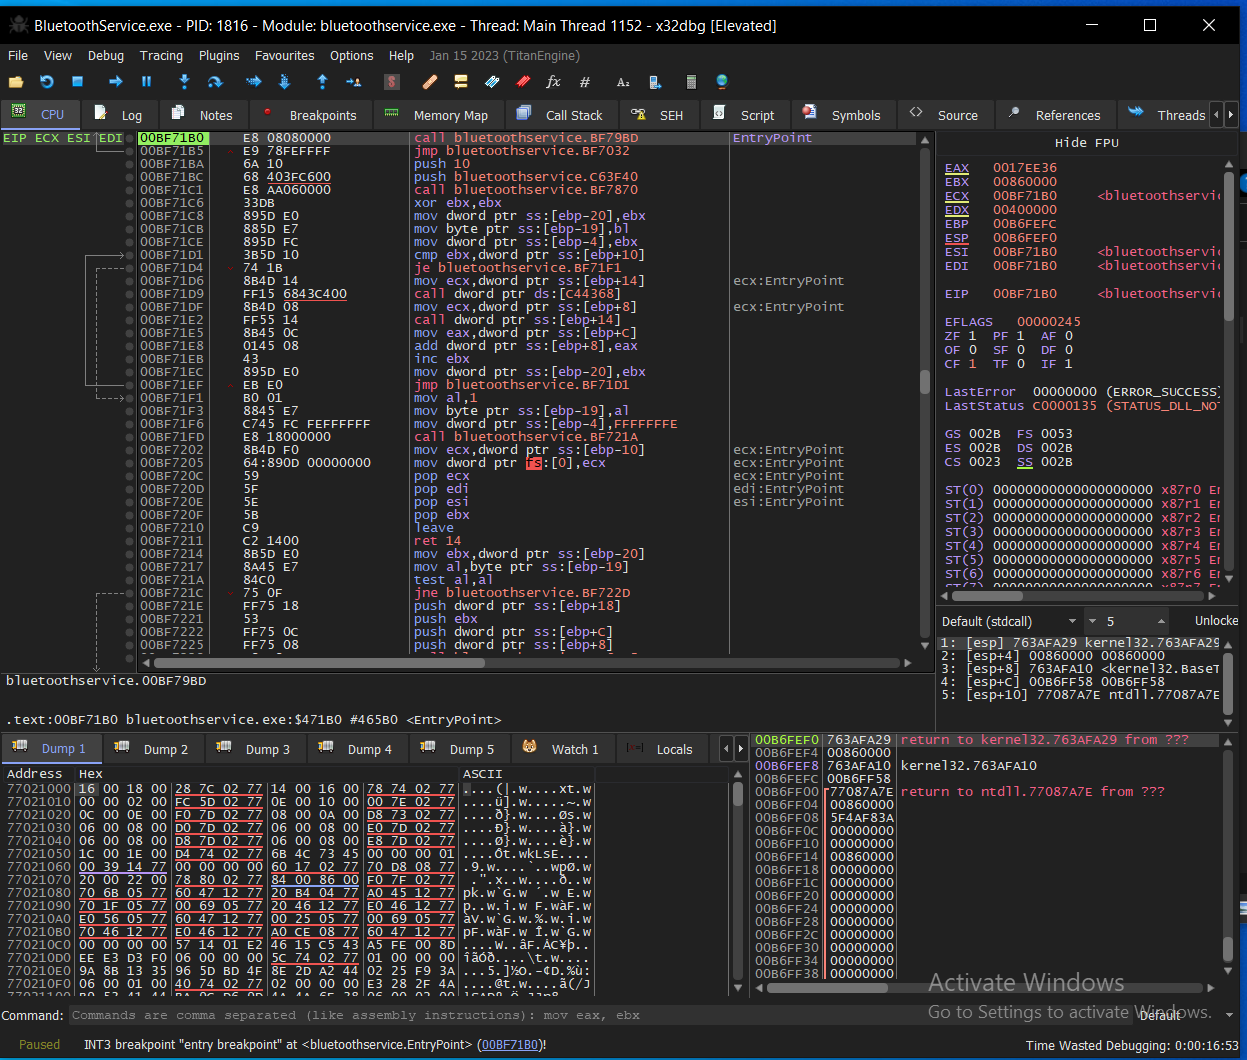
\includegraphics[width=0.85\textwidth]{img/EntryPoint_BluetoothServiceexe.png}
  \caption{Entry Point di \texttt{BluetoothService.exe}}
\end{figure}

\subsubsection*{Sintesi dei Tentativi e degli Ostacoli Incontrati}
L'estrazione del payload ha richiesto il superamento di molteplici tecniche di evasione implementate dall'APT Lotus Blossom. Di seguito i passaggi fondamentali del diario di analisi:

\begin{enumerate}
  \item \textbf{Evasione Iniziale (Bait and Switch)}: I primi tentativi di usare Software Breakpoints sulle API standard e ScyllaHide si sono rivelati inefficaci. Il malware, una volta rilevato il debugger, clona se stesso in background ed evade l'analisi terminando il processo principale.
  \begin{figure}[H]
    \centering
    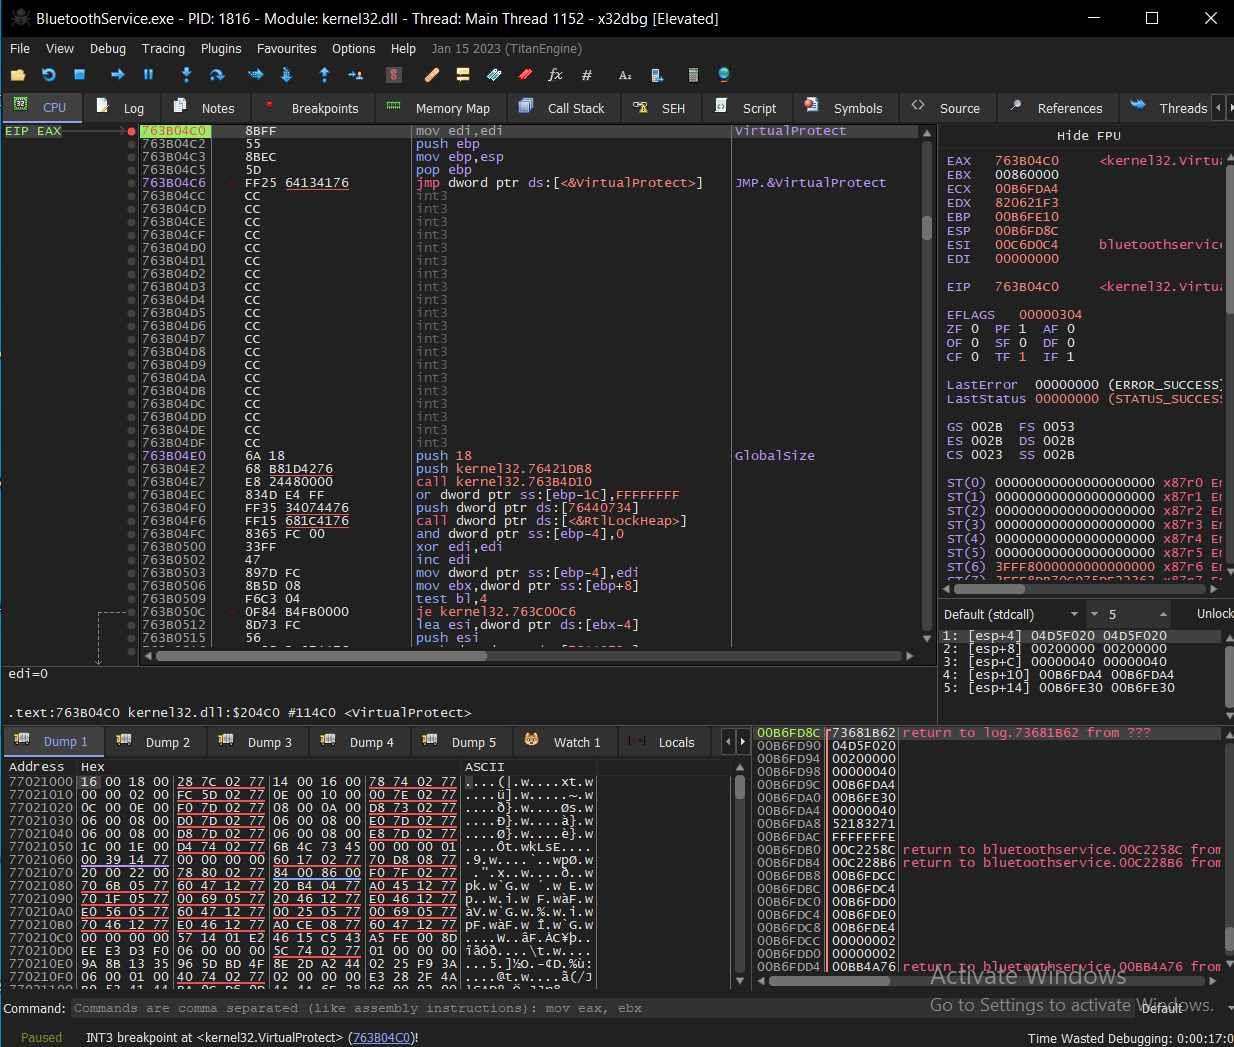
\includegraphics[width=0.85\textwidth]{img/BreakPoint_VirtualProtect.png}
    \caption{Breakpoint su \texttt{VirtualProtect}}
  \end{figure}

  \item \textbf{Esecuzione Precoce in DllMain}: Un'analisi architetturale ha rivelato che il codice malevolo non attende il raggiungimento dell'Entry Point ufficiale dell'eseguibile, ma si innesca direttamente nella \texttt{DllMain} appena \texttt{log.dll} viene caricata in memoria. È stato quindi necessario riconfigurare x32dbg per intercettare l'esecuzione "User DLL Entry".
  \begin{figure}[H]
    \centering
    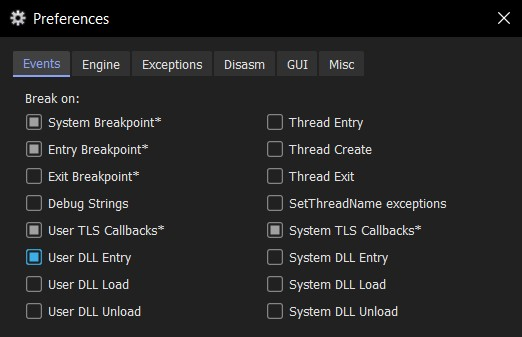
\includegraphics[width=0.7\textwidth]{img/x32dgb_preferences.jpg}
    \caption{Preferenze x32dbg}
  \end{figure}
  \begin{figure}[H]
    \centering
    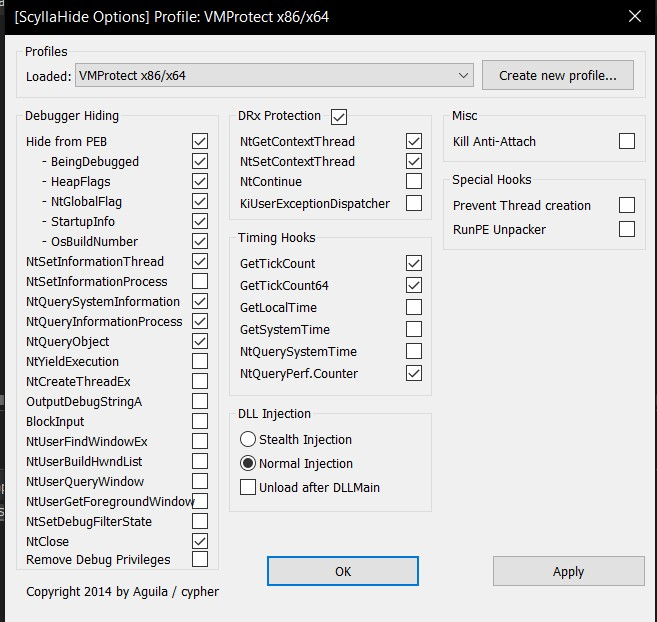
\includegraphics[width=0.7\textwidth]{img/scyllahide_opt.jpg}
    \caption{Opzioni ScyllaHide}
  \end{figure}

  \item \textbf{Trappole nella Memoria e False Piste (Decoy PE)}: Tramite Hardware Breakpoints su API native (come \texttt{ZwProtectVirtualMemory}), si è isolato un eseguibile in memoria. La sua ricostruzione (tramite PE-bear per correggere i Section Headers) ha però svelato un Decoy PE (esca), di dimensioni esigue e privo di codice Assembly utile.
  \begin{figure}[H]
    \centering
    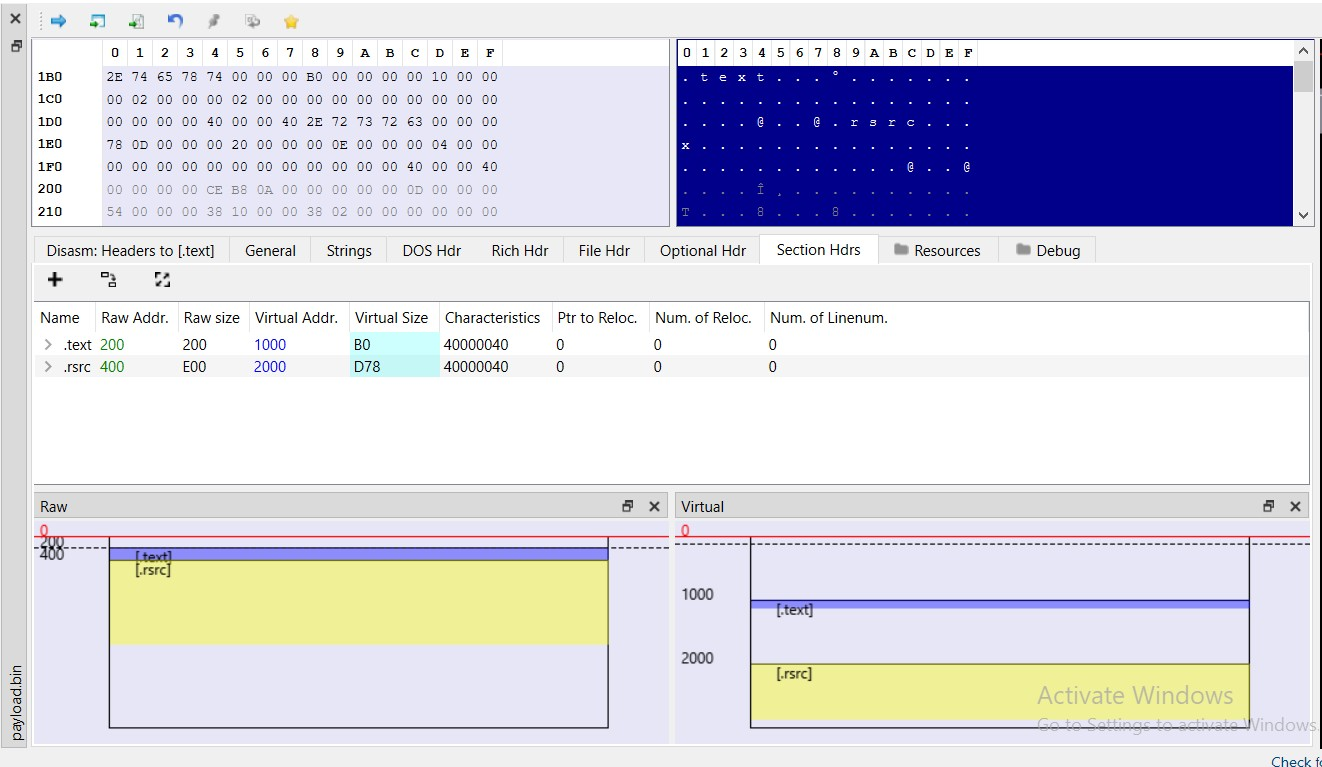
\includegraphics[width=0.7\textwidth]{img/section_headers.jpg}
    \caption{Section Headers in PE-bear}
  \end{figure}
  \begin{figure}[H]
    \centering
    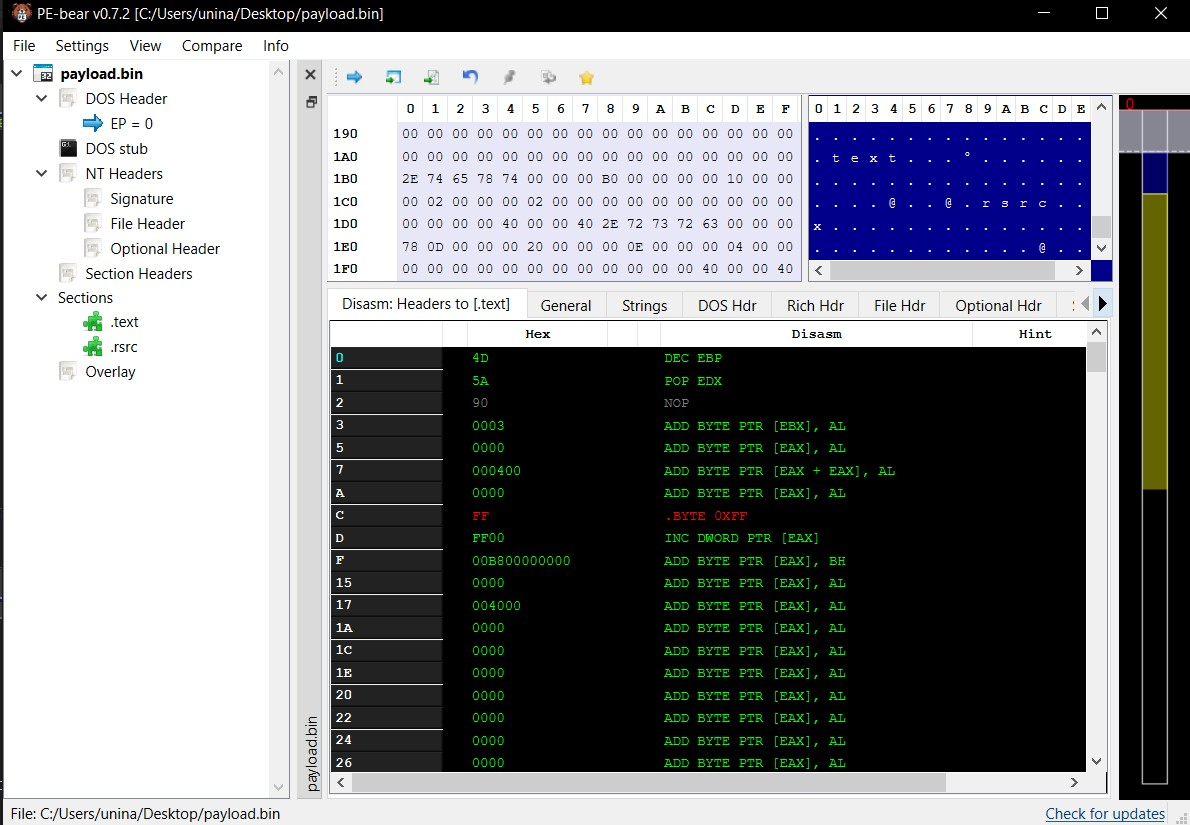
\includegraphics[width=0.7\textwidth]{img/PE.jpg}
    \caption{PE non valido dumpato}
  \end{figure}
  \begin{figure}[H]
    \centering
    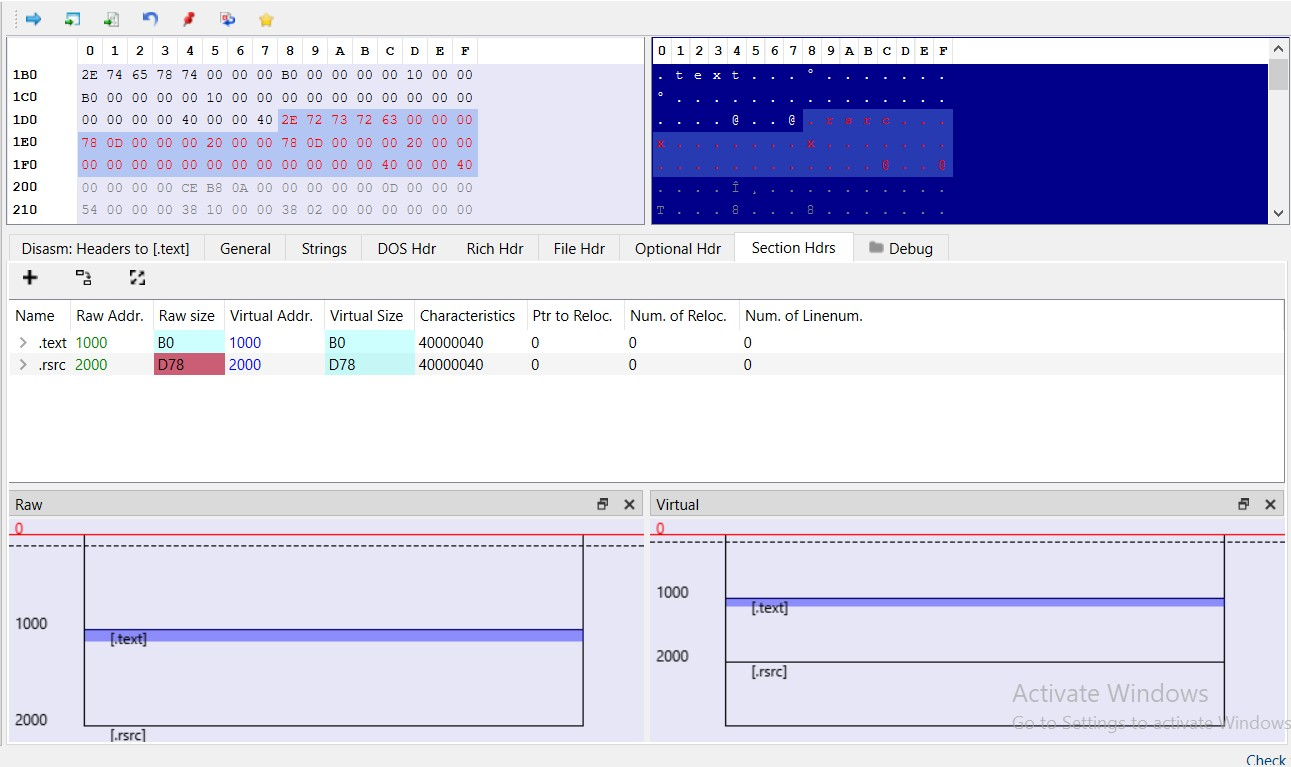
\includegraphics[width=0.7\textwidth]{img/PE_fixed.jpg}
    \caption{PE corretto con PE-bear}
  \end{figure}

  \item \textbf{Bypass dell'API Hashing}: L'abbandono temporaneo dell'analisi dinamica a favore di quella statica in IDA ha permesso di scoprire l'utilizzo di API Hashing (FNV-1a modificato).
  \begin{figure}[H]
    \centering
    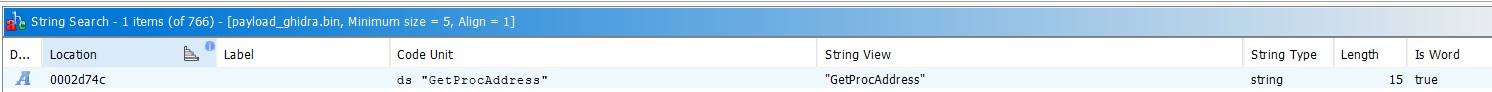
\includegraphics[width=0.7\textwidth]{img/lib.jpg}
    \caption{Risoluzione dinamica delle librerie}
  \end{figure}

  \item \textbf{Tracking Dinamico ed Estrazione}: Conoscendo la logica, si sono impostati breakpoint mirati in x32dbg sulle routine di decrittazione, permettendo il dump finale dello shellcode, il quale decritta il file usando una logica XOR custom e la chiave \texttt{gQ2JR\&9;}.
  \begin{figure}[H]
    \centering
    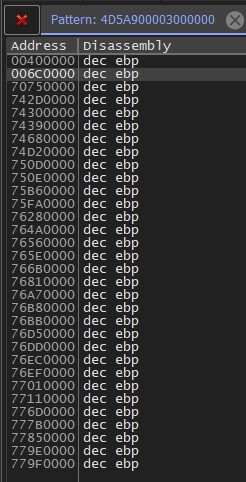
\includegraphics[width=0.7\textwidth]{img/memory_map.jpg}
    \caption{Memory Map dello shellcode in RAM}
  \end{figure}
\end{enumerate}

\begin{figure}[H]
  \centering
  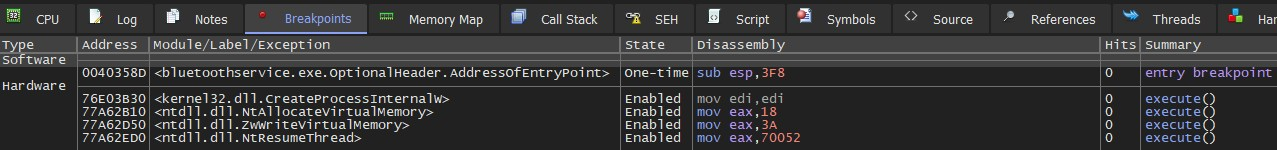
\includegraphics[width=0.85\textwidth]{img/breakpoint.jpg}
  \caption{Breakpoint sulle routine di decrittazione}
\end{figure}

\begin{figure}[H]
  \centering
  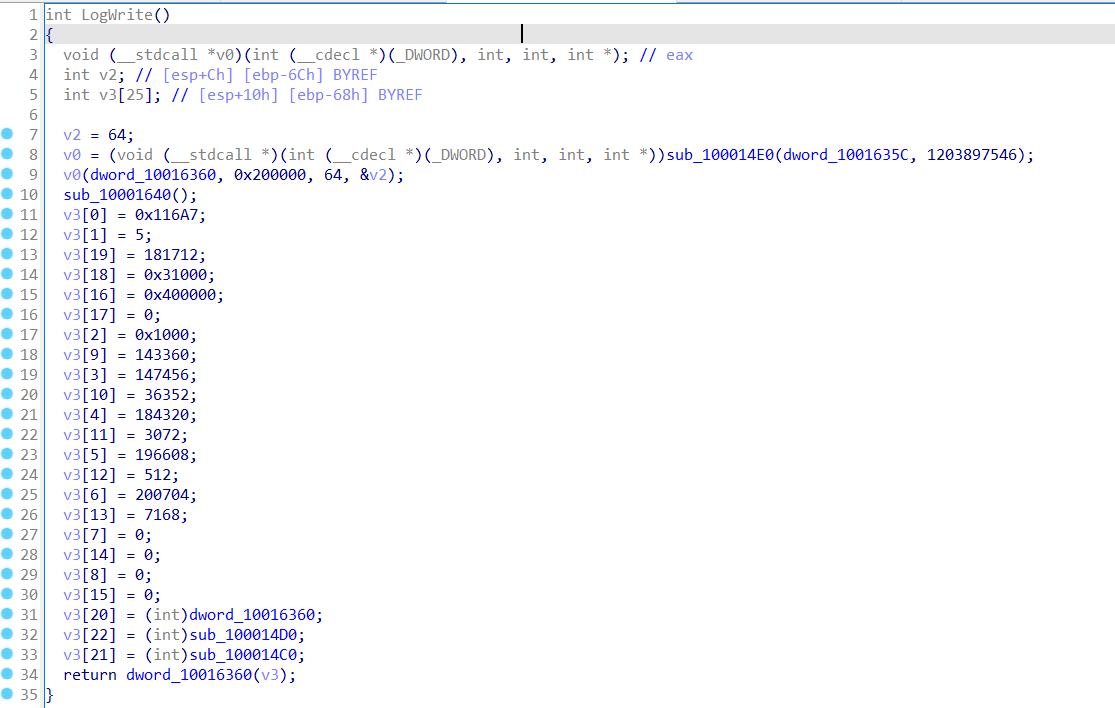
\includegraphics[width=0.85\textwidth]{img/logWrite.png}
  \caption{Codice decompilato di \texttt{LogWrite}}
\end{figure}

\subsection{Architettura del Modulo Principale (Chrysalis Backdoor)}
Dopo aver estratto con successo lo shellcode, è stato possibile analizzarlo. La prima operazione che viene eseguita è il caricamento delle librerie mediante un'operazione di hashing più complessa rispetto a quella vista all'interno di \texttt{LogWrite}.

\begin{figure}[H]
  \centering
  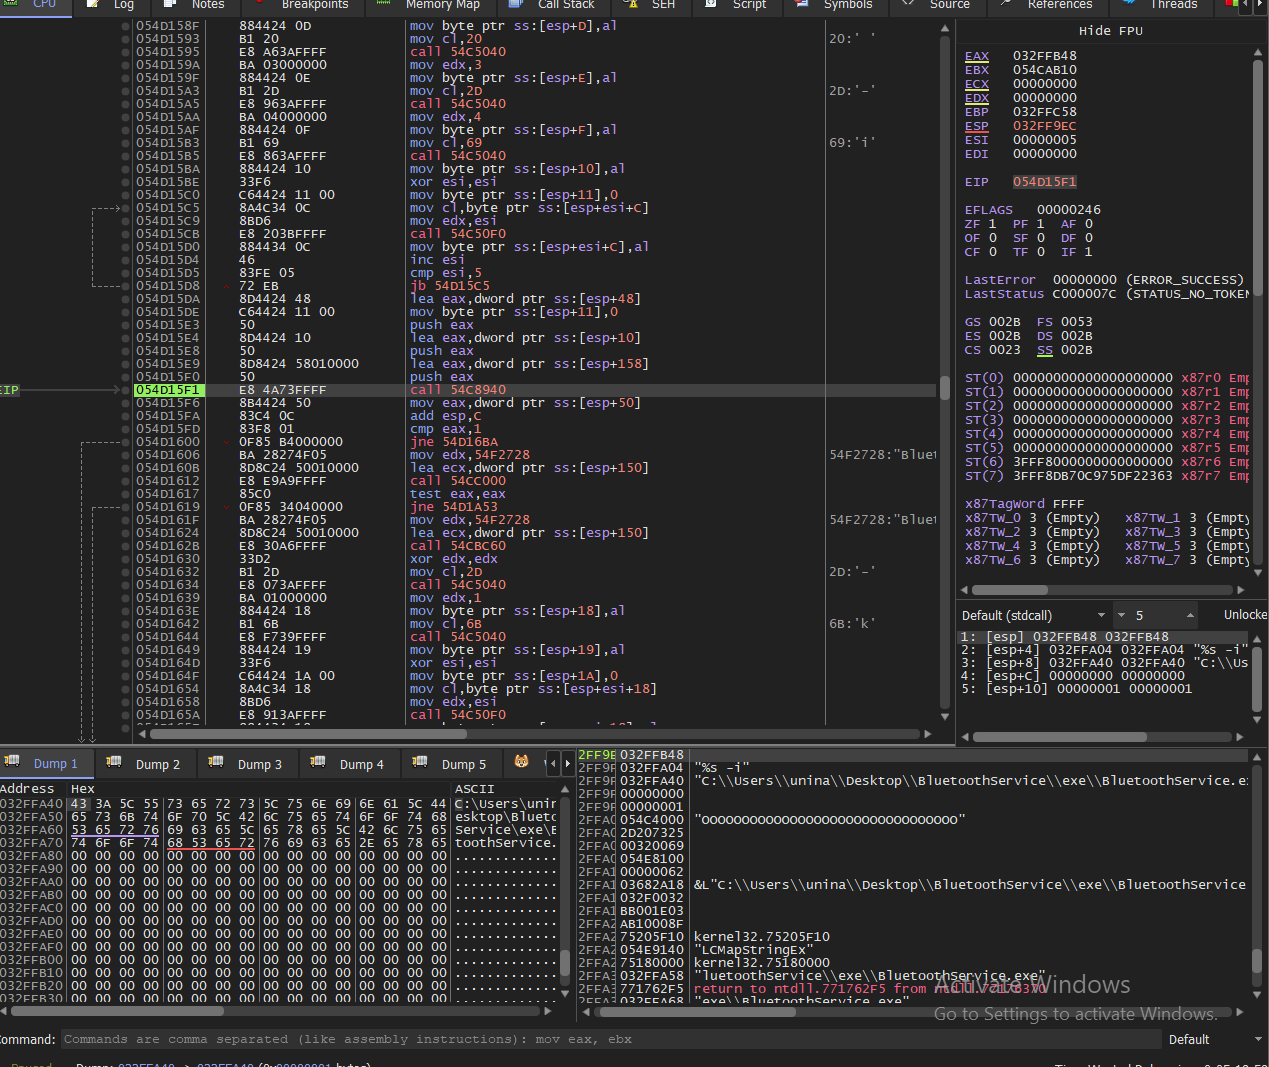
\includegraphics[width=0.85\textwidth]{img/Execution_ShellCode.png}
  \caption{Esecuzione dello Shellcode in IDA}
\end{figure}

\subsubsection{Decrittazione della Configurazione e Destinazione C2}
Successivamente, viene decrittata una zona di memoria che ospita al suo interno i parametri per una richiesta HTTP all'esterno. L'algoritmo crittografico utilizzato per questo blocco è \textbf{RC4}, impiegando la chiave hardcodata \texttt{qwhvb\textasciicircum 435h\&*7}, la quale viene caricata all'interno carattere per carattere per evadere i controlli sulle stringhe.

\begin{figure}[H]
  \centering
  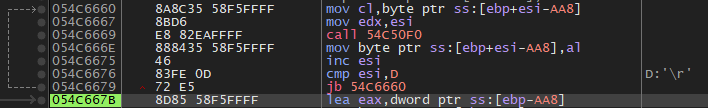
\includegraphics[width=0.7\textwidth]{img/routine_extract_key.png}
  \caption{Routine di estrazione chiave config}
\end{figure}
\begin{figure}[H]
  \centering
  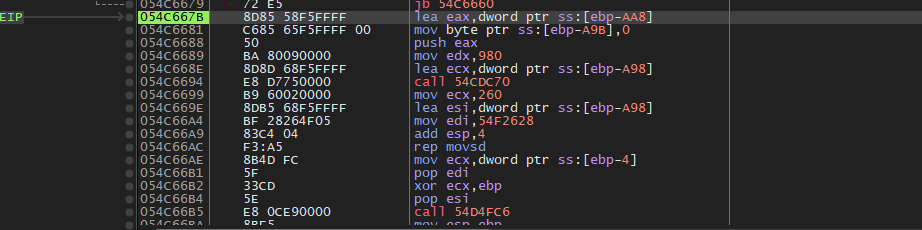
\includegraphics[width=0.7\textwidth]{img/routine_decrypt.png}
  \caption{Routine RC4 Decrypt}
\end{figure}
\begin{figure}[H]
  \centering
  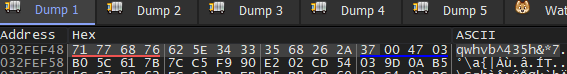
\includegraphics[width=0.7\textwidth]{img/rc4_key.png}
  \caption{Chiave RC4 in memoria}
\end{figure}

Una volta decifrata la configurazione, il malware svela il dominio del Command and Control (C2):
\begin{itemize}
  \item \textbf{URL di Esfiltrazione}: \url{https://api.skycloudcenter.com/a/chat/s/70521ddf-a2ef-4adf-9cf0-6d8e24aaa821}
  \item Possiamo notare anche l'indirizzo IP \textbf{\texttt{61.4.102.97}}.
\end{itemize}

In questo modo siamo riusciti a risalire all'URL di esfiltrazione individuato nelle fasi iniziali.

\subsubsection{Tripla Modalità di Esecuzione}
Chrysalis implementa una logica differenziata a tre vie basata sugli argomenti a riga di comando passati all'eseguibile, con lo scopo di eludere sandbox o controlli statici e instaurare la persistenza in modo silente.

\begin{enumerate}
  \item \textbf{Modalità Installazione (Nessun parametro)}:
  Crea un servizio di sistema o una voce di registro in modo da assicurare la persistenza all'avvio dell'host. Questo servizio esegue il malware passandogli specificamente il parametro \texttt{-i}. Completata l'installazione, il processo originario termina immediatamente.
  \begin{figure}[H]
    \centering
    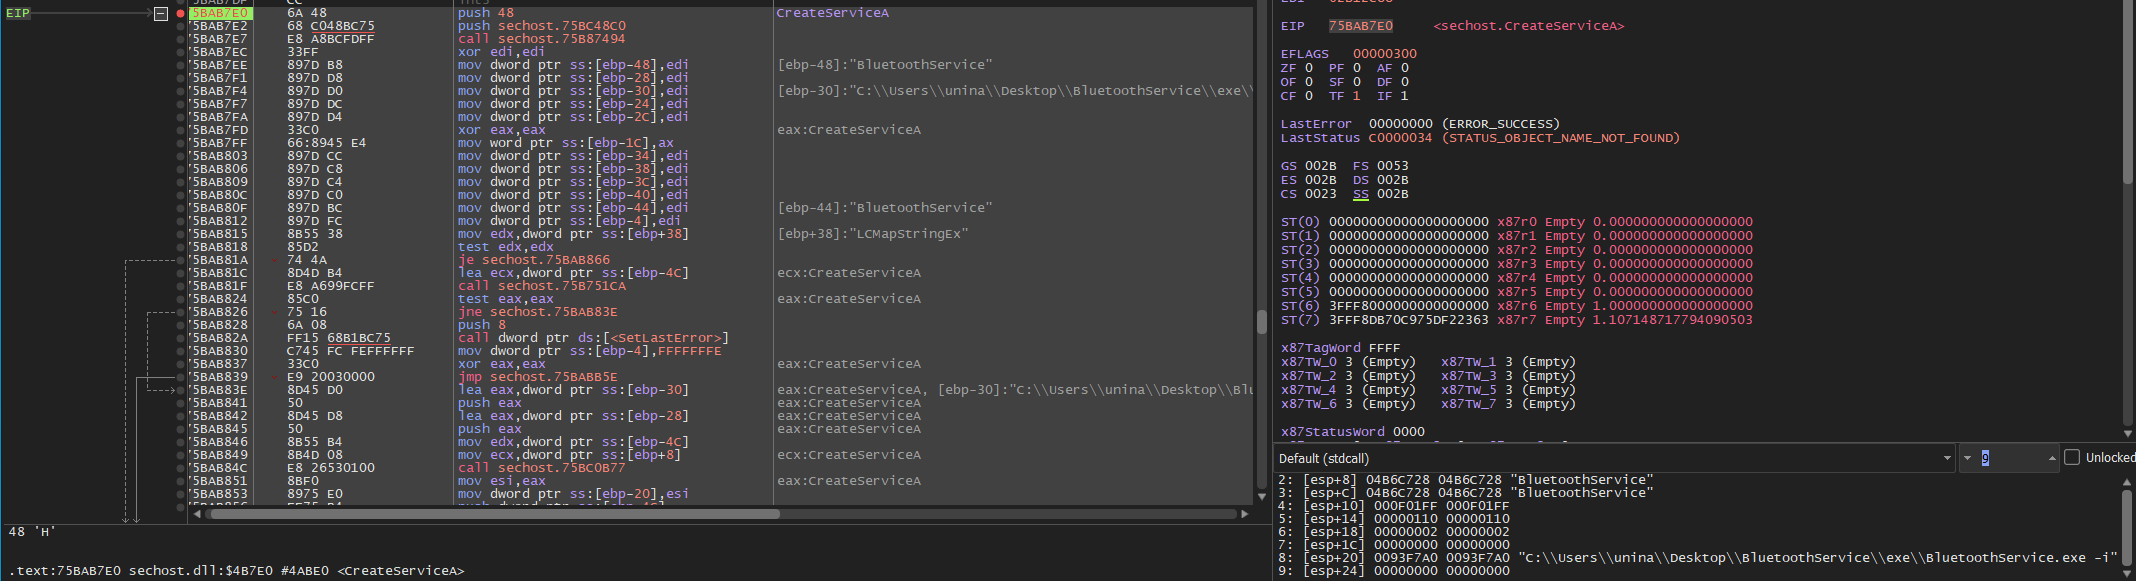
\includegraphics[width=0.7\textwidth]{img/CreateService_Persistence.png}
    \caption{Creazione del servizio persistente}
  \end{figure}

  \item \textbf{Modalità Launcher (Parametro \texttt{-i})}:
  Genera e lancia in background una nuova istanza di se stesso tramite la funzione di sistema \texttt{ShellExecuteA}, iniettandovi il parametro \texttt{-k}. In questo modo elude il tree genitore.
  \begin{figure}[H]
    \centering
    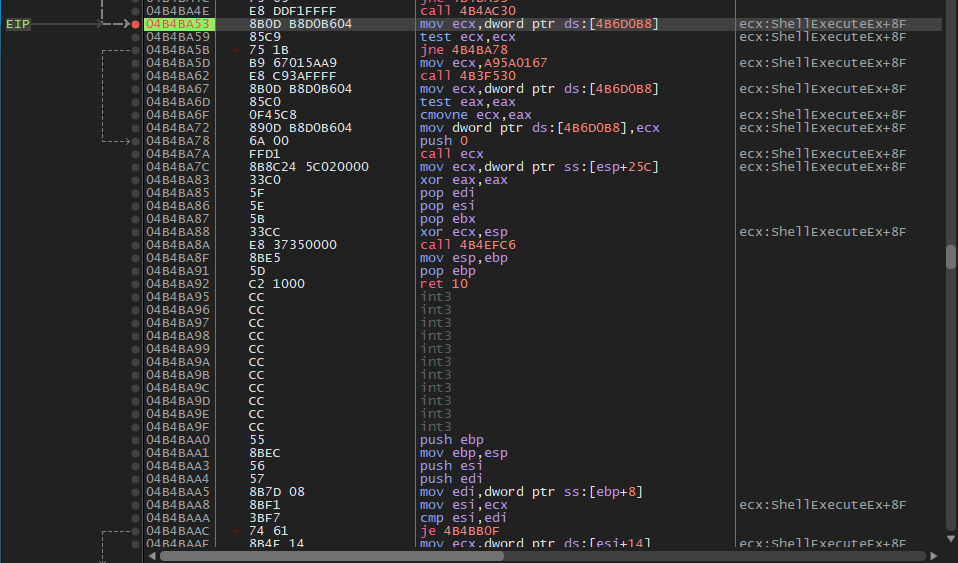
\includegraphics[width=0.7\textwidth]{img/ShellExecute_func.png}
    \caption{Funzione di caricamento ShellExecute}
  \end{figure}
  \begin{figure}[H]
    \centering
    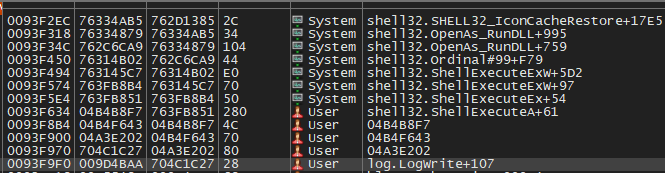
\includegraphics[width=0.7\textwidth]{img/ShellExecute.png}
    \caption{Parametri di ShellExecute}
  \end{figure}

  Tramite Process Explorer possiamo osservare il processo figlio che viene creato:
  \begin{figure}[H]
    \centering
    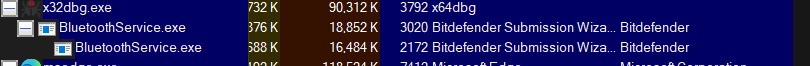
\includegraphics[width=0.7\textwidth]{img/BluetoothServicesSpawn.png}
    \caption{Processo figlio spawnato}
  \end{figure}

  \item \textbf{Modalità Payload (Parametro \texttt{-k})}:
  Questa modalità salta i controlli preliminari e avvia direttamente la logica malevola finale, decodificando e mandando in esecuzione il codice (Shellcode + comunicazione C2).
\end{enumerate}

\begin{itemize}
  \item \textbf{Creazione Mutex}: Verifica la presenza di un Mutex (es. \texttt{Global\textbackslash Jdhfv\_1.0.1}) e in caso contrario lo crea per segnalare la sua singola istanza attiva.
  \begin{figure}[H]
    \centering
    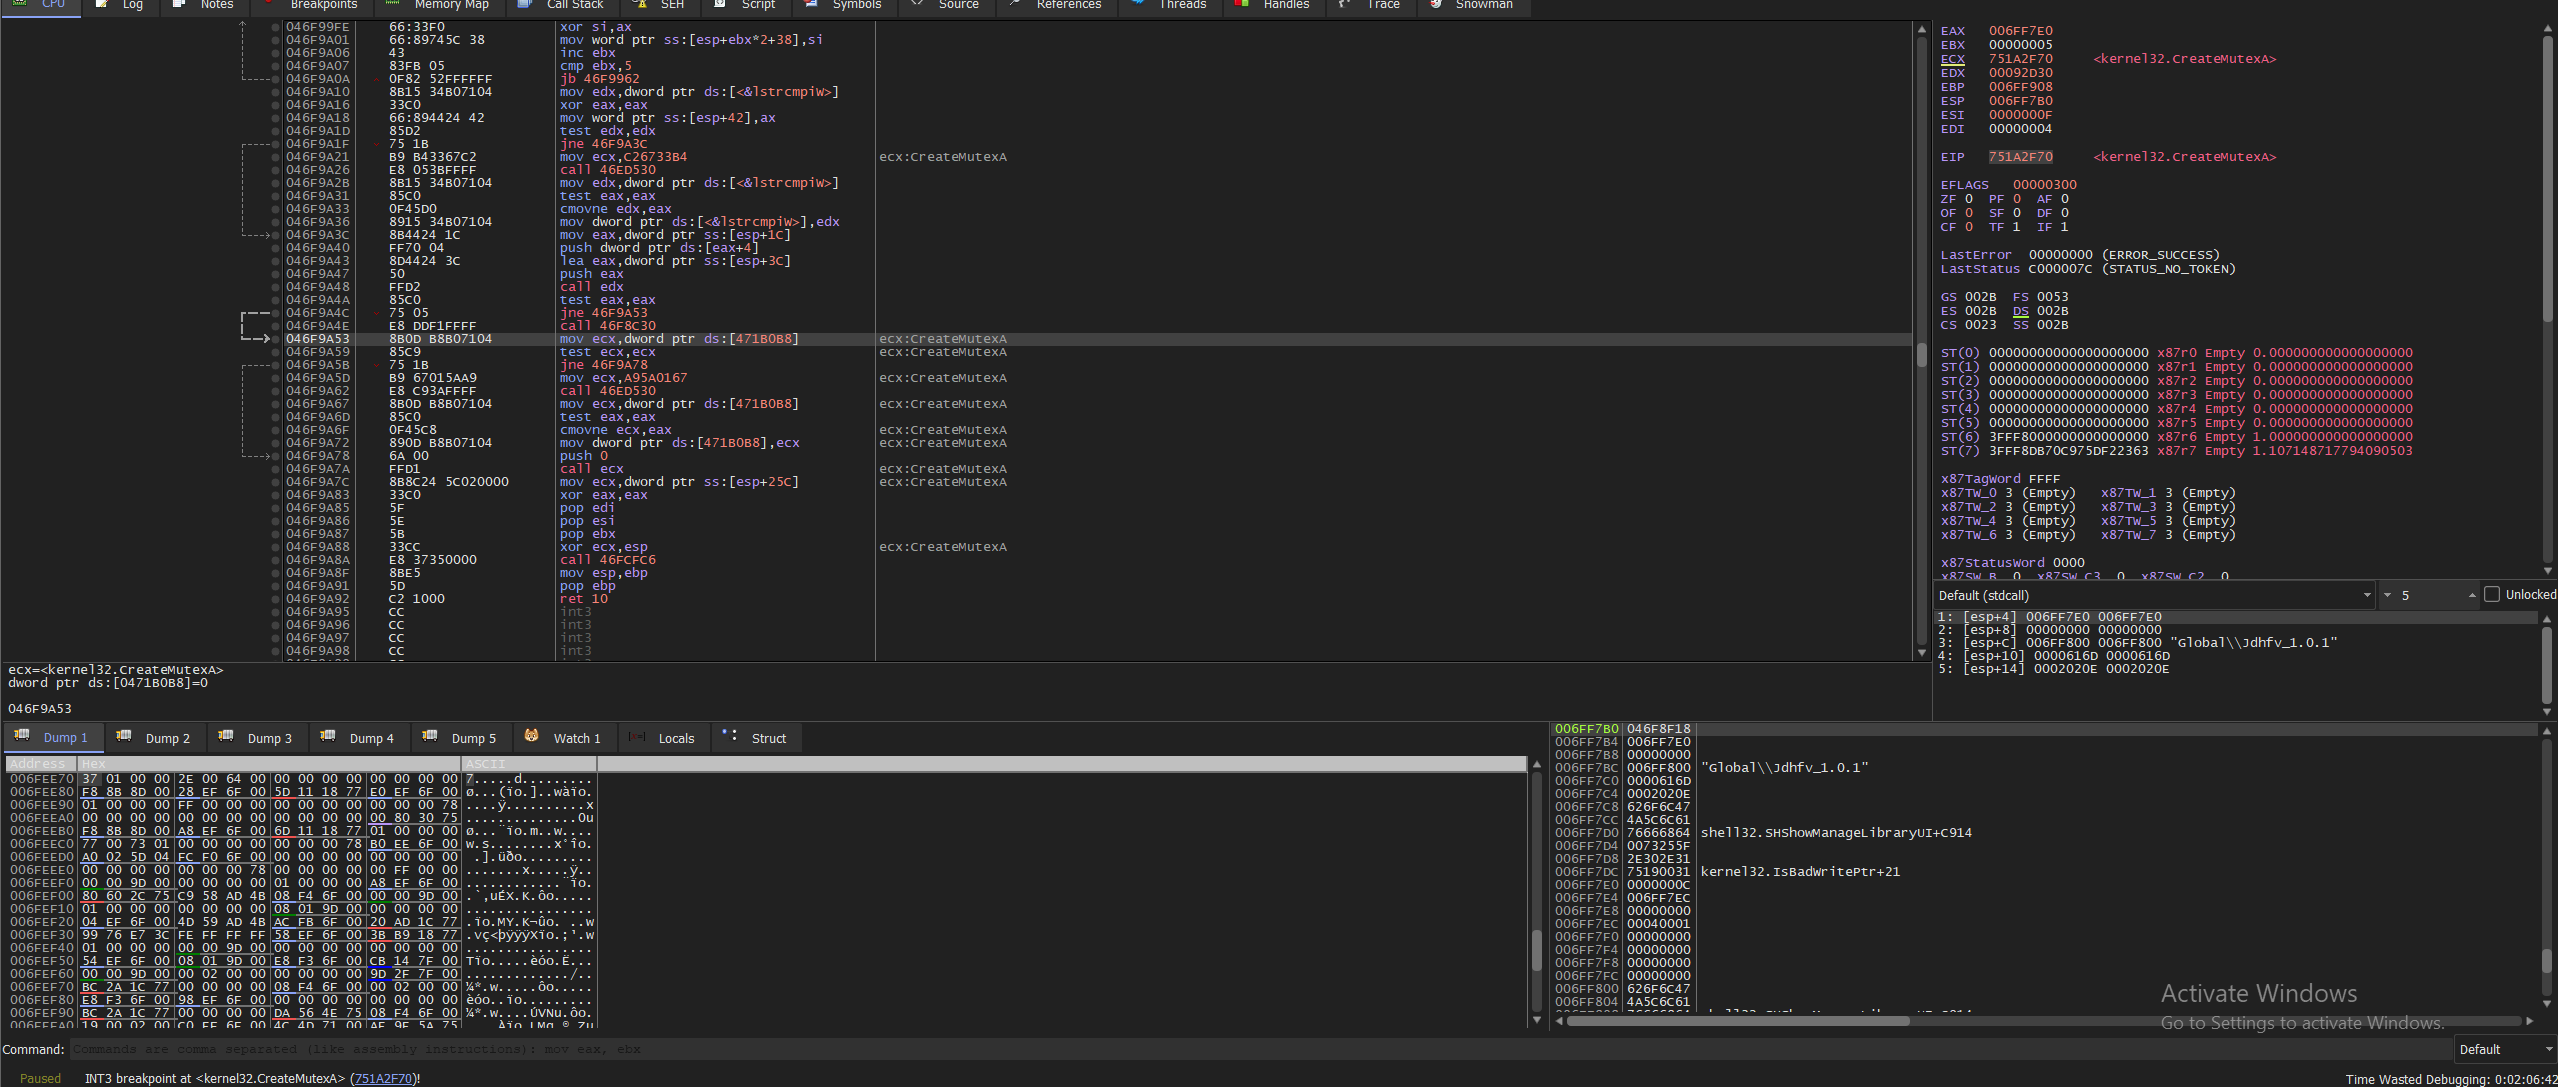
\includegraphics[width=0.7\textwidth]{img/StackNameMutex.png}
    \caption{Stack per la creazione del Mutex (parte 1)}
  \end{figure}
  \begin{figure}[H]
    \centering
    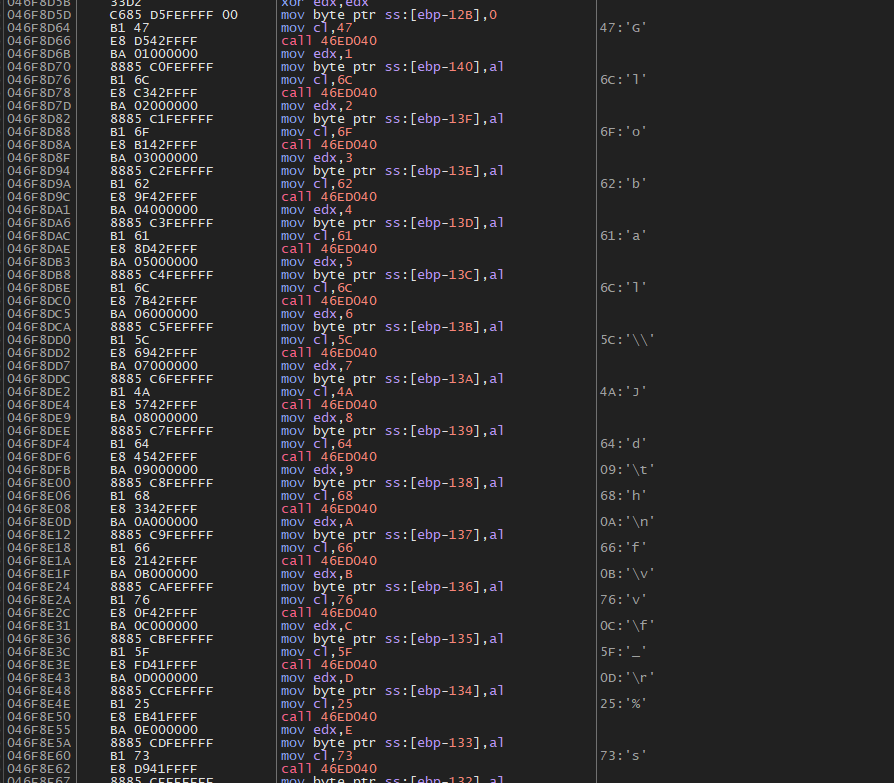
\includegraphics[width=0.7\textwidth]{img/Stack_NameMutex2.png}
    \caption{Stack per la creazione del Mutex (parte 2)}
  \end{figure}

  Questo inoltre può essere confermato anche tramite Process Explorer:
  \begin{figure}[H]
    \centering
    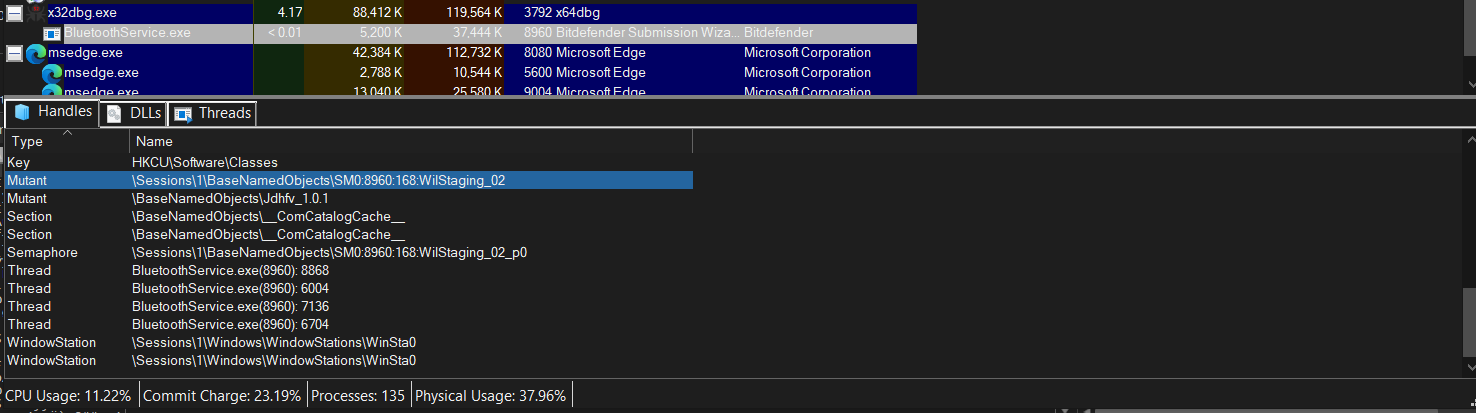
\includegraphics[width=0.7\textwidth]{img/procexp_mutant.png}
    \caption{Visualizzazione Mutex in Process Explorer}
  \end{figure}

  \item \textbf{Info Stealing}: Raccoglie una fingerprint approfondita dell'host, comprendente i dettagli del Sistema Operativo, l'elenco degli Antivirus, l'orario e il Nome Utente/Computer. È inoltre possibile notare che lo stack contiene i vari metodi HTTP delle richieste.
  \begin{figure}[H]
    \centering
    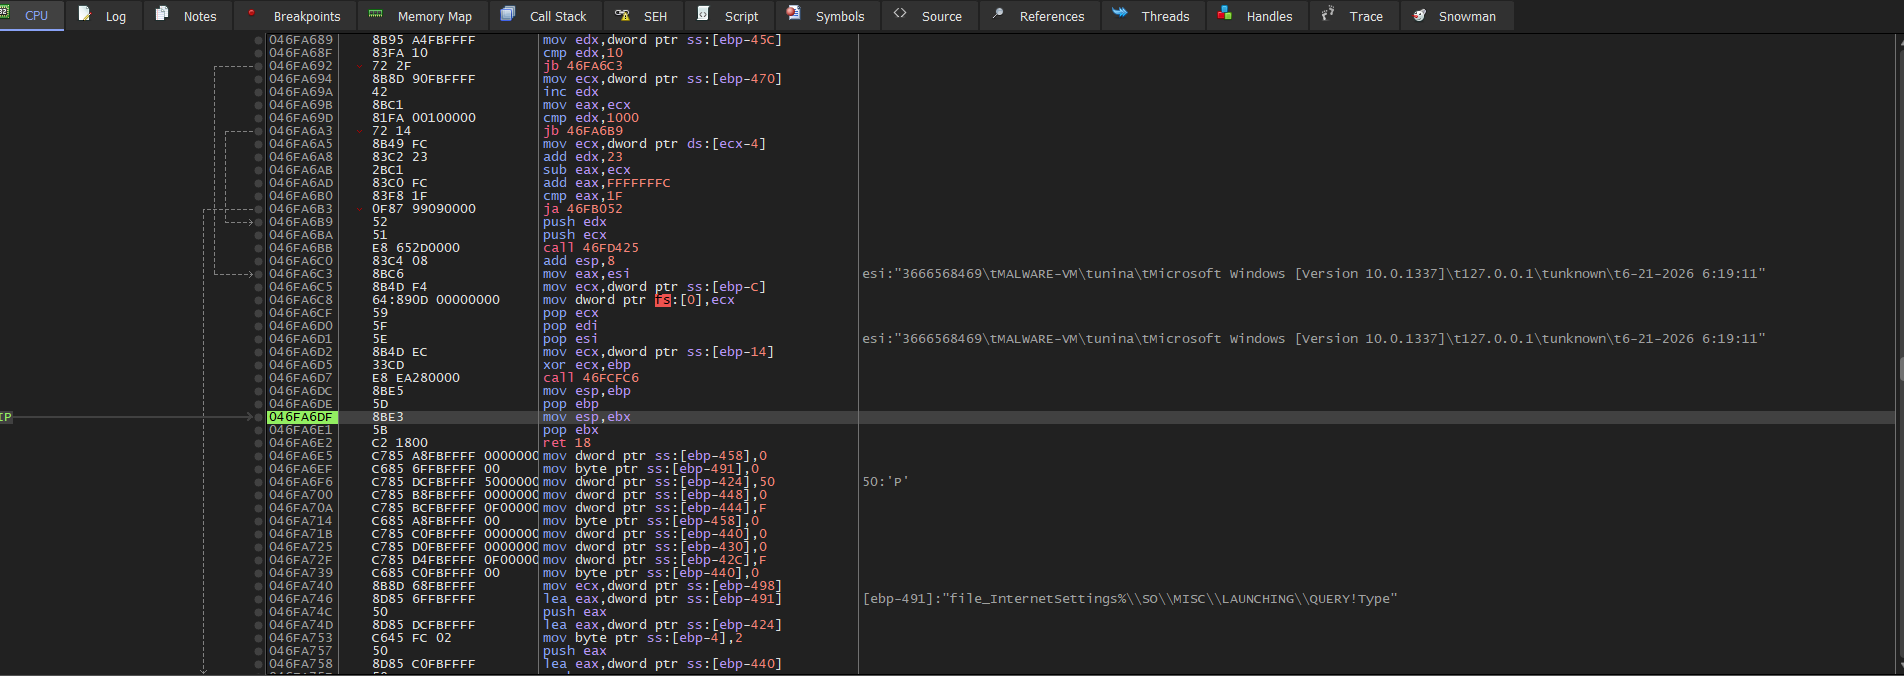
\includegraphics[width=0.7\textwidth]{img/infoStealer.png}
    \caption{Informazioni raccolte in memoria}
  \end{figure}
  \begin{figure}[H]
    \centering
    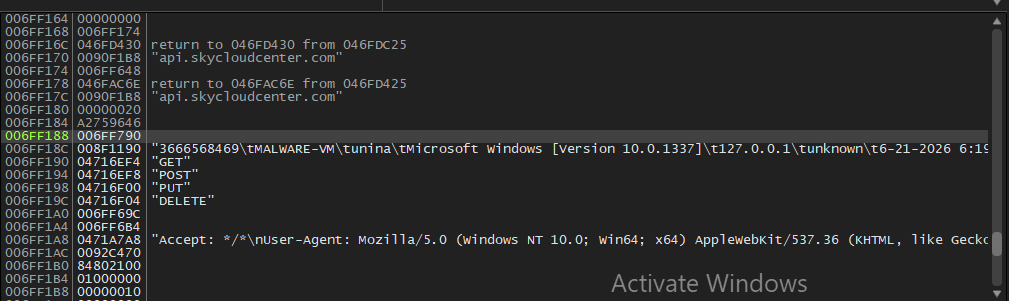
\includegraphics[width=0.7\textwidth]{img/StackInfoStealer.png}
    \caption{Stack relativo all'Info Stealer}
  \end{figure}

  \item \textbf{Connessione C2 e Terminale Interattivo}: Aggrega i dati raccolti, calcola l'hash FNV-1a come UUID e li cifra nuovamente usando un'altra chiave RC4 (\texttt{vAuig34\%}\textbackslash textasciicircum\texttt{325hGV}). Successivamente, instaura un terminale/canale bidirezionale (in stile reverse shell cmd.exe) che trasmette costantemente dati all'indirizzo C2 appena decrittato avvalendosi di richieste in formato \textbf{HTTP POST}.
  \begin{figure}[H]
    \centering
    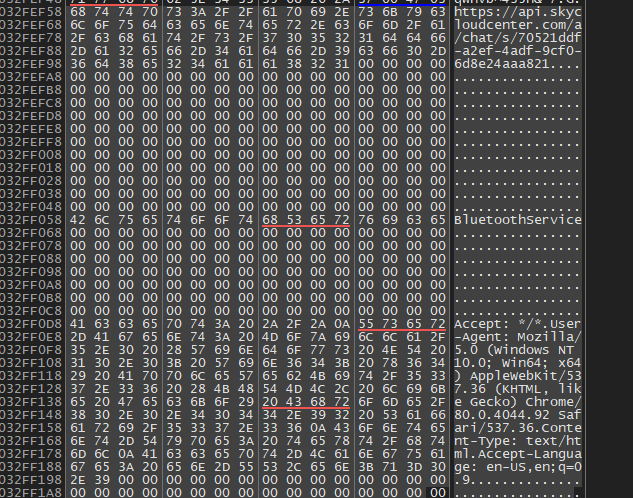
\includegraphics[width=0.85\textwidth]{img/webrequest_header.png}
    \caption{Web Request Header HTTP POST}
  \end{figure}
  \begin{figure}[H]
    \centering
    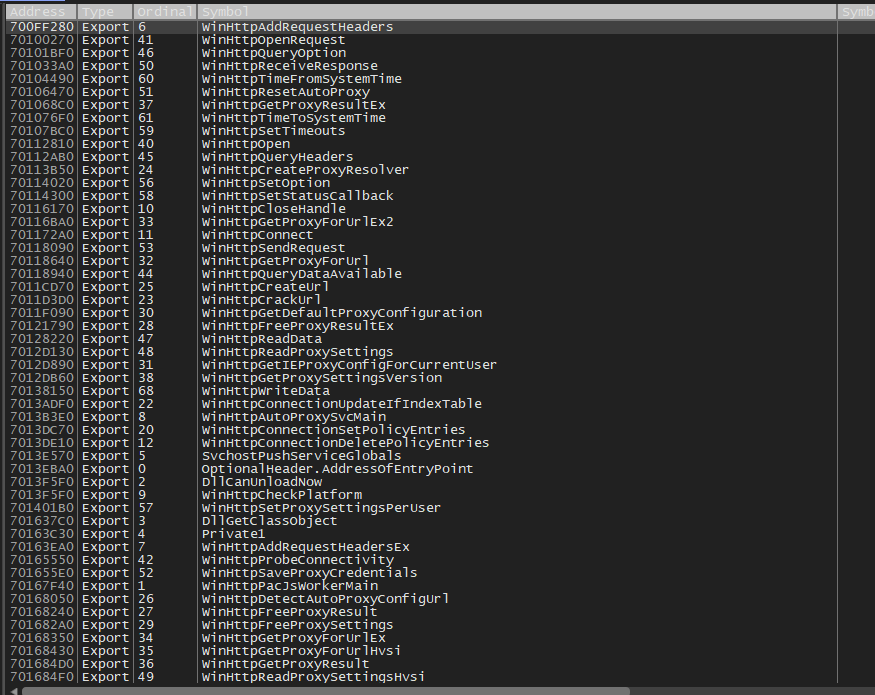
\includegraphics[width=0.85\textwidth]{img/LibCaricate_Http.png}
    \caption{Librerie HTTP Caricate}
  \end{figure}
\end{itemize}

Tramite questo canale interattivo su protocollo POST, la backdoor Chrysalis può ricevere ed eseguire autonomamente una suite di 16 diverse istruzioni (upload, download, proxy e spawn di processi), confermandosi uno strumento altamente modulare ed evasivo per il toolkit Lotus Blossom.
